\documentclass[output=paper,colorlinks,citecolor=brown]{langscibook}
\ChapterDOI{10.5281/zenodo.19708149}
\author{Mitchell Browne\orcid{0000-0001-7623-8179}\affiliation{Macquarie University; University of Western Australia} and         Thomas Ennever\orcid{0000-0003-4838-4122}\affiliation{University of Surrey} and         David Osgarby\orcid{0000-0002-5250-2438}\affiliation{University of Glasgow}} \title{The grammatical realisation of apprehensional functions in Ngumpin-Yapa languages (Australia)}
\shorttitlerunninghead{Apprehensional functions in Ngumpin-Yapa languages (Australia)}

\abstract{This paper provides a survey of apprehension constructions in the Ngumpin-Yapa (Pama-Nyungan) languages of northern Australia. As in many Australian languages, there are morphosyntactically distinct strategies for encoding apprehension in Ngumpin-Yapa languages: a verbal \textit{apprehensional} morpheme and a nominal \textit{aversive} morpheme. Languages differ in terms of the extent to which these morphemes uniquely encode apprehension, some also encoding physical location or potentiality. We survey apprehensional morphemes in nine Ngumpin-Yapa languages: Walmajarri, Ngardi, Jaru, Wanyjirra, Gurindji, Bilinarra, Mudburra, Warlmanpa and Warlpiri. In these Ngumpin-Yapa languages, the verbal apprehensional morphemes are found in the auxiliary complex as a base for bound pronominals. The nominal aversive morphemes are oblique case suffixes that relate nominals and nominalised predicates to main predicates. The auxiliary bases form part of the system of finite tense–aspect–modality, whereas the case suffixes act as complementisers for non-finite clauses, with dependent tense features. Both classes of morphemes can appear in independent and dependent syntactic environments. Additionally, both classes of apprehensional morphemes can have non-apprehensional functions, for example in Wanyjirra the comitative case suffix introduces concomitant participants, which can also be used to express aversion to particular participants. This chapter makes a substantive contribution to our understanding of apprehension in Australian languages -- a topic that hitherto has received little attention, despite the prevalence of apprehensional morphemes in Australian languages. This survey highlights the fact that even in a group of closely related languages, the grammatical encoding of undesirability can vary greatly.
}

%move the following commands to the "local..." files of the master project when integrating this chapter

%\usepackage[table,xcdraw]{xcolor}


\IfFileExists{../localcommands.tex}{
   \addbibresource{../localbibliography.bib}
   \usepackage{tabularx,multicol}
\usepackage{url}
\urlstyle{same}

\usepackage{langsci-optional}
\usepackage{langsci-lgr}
\usepackage{langsci-gb4e}

\babelprovide[import]{hebrew}

\usepackage{paralist} %%may not be needed, currently used in questionnaire


%Siena added packages for introduction; not sure they are needed
\usepackage[normalem]{ulem}
\useunder{\uline}{\ul}{}

%from Treis:
\usepackage{listings}
\lstset{basicstyle=\ttfamily,tabsize=2,breaklines=true}

%%from Francez
% % % \usepackage{cjhebrew}
%\usepackage{tipa}  Also included by D&A, need to check with LSP whether to change it to language science tipa
\usepackage{leipzig}
%%from Dabkowski&AnderBois:

\usepackage[shortlabels]{enumitem} 
\usepackage{centernot}
\usepackage{arydshln}
\usepackage{newunicodechar}
\usepackage{csquotes}
%\let\sups\relax \usepackage{tipa} commented out on 7/3/25 Martina
% \usepackage[all]{nowidow}
\usepackage{listings} \lstset{basicstyle=\ttfamily}
\usepackage{multirow}
\usepackage{rotating}
\usepackage{pdflscape}
\usepackage{xspace}
%\usepackage{tabularx}
%\usepackage{multicol}
\usepackage{supertabular}
\usepackage{hhline}
\usepackage{bbding} %this package is for the checkmarks in Table 6 in Browne et al.

%\usepackage{qtree}
%\usepackage{tree-dvips}

\usepackage{array}
\usetikzlibrary{calc,tikzmark,matrix}
\usepgflibrary{shadings}
\usepackage{pifont}
%from Fedotov:

\usepackage{langsci-textipa}
%\usepackage{multirow}


%\usepackage{xeCJK}

%%%%%%%%%%%%%%%%%%%%%%%%%%%%%%%%%%%%%%%%%%%%%%%%%%%%
%%% EXAMPLES %%%%%%%%%%%%%%%%%%%%%%%%%%%%%%%%%%%%%%%
%%%%%%%%%%%%%%%%%%%%%%%%%%%%%%%%%%%%%%%%%%%%%%%%%%%% 

% if you want the source line of examples to be in
% italics, uncomment the following line
\renewcommand{\exfont}{\itshape}
% to add additional information to the right of
% examples, uncomment the following line

%\usepackage{langsci/styles/jambox}


%%% FOOTNOTE EXAMPLE NUMBERING
% \makeatletter
% \patchcmd{\@footnotetext}{\setcounter{fnx}{0}}{\renewcommand{\thexnumi}{\roman{xnumi}}}{}{}
% \apptocmd{\@footnotetext}{
%     \@noftnotetrue
%     \renewcommand{\thexnumi}{\arabic{xnumi}}%
% }{}{}
%
% \makeatother
\usepackage[linguistics,edges]{forest}
\usepackage{hyphenat}
\usepackage{langsci-branding}

   \makeatletter
\let\thetitle\@title
\let\theauthor\@author
\makeatother

\newcommand{\togglepaper}[1][0]{
   \bibliography{../localbibliography}
   \papernote{\scriptsize\normalfont
     \theauthor.
     \titleTemp.
    To appear in:
    Martina Faller,  Marine Vuillermet \&  Eva Schultze-Berndt (eds.). Apprehensional Constructions in a cross-linguistic perspective. Berlin: Language Science Press. [preliminary page numbering]
   }
   \pagenumbering{roman}
   \setcounter{chapter}{#1}
   \addtocounter{chapter}{-1}
}

\newbool{bookcompile}
\booltrue{bookcompile}
\newcommand{\bookorchapter}[2]{\ifbool{bookcompile}{#1}{#2}}


\newfontfamily\FedotovBoldEmptySetFont{LibertinusSerif-Italic.otf}[AutoFakeBold=2.5]
\newcommand{\FedotovBoldEmpty}{{\FedotovBoldEmptySetFont\bfseries ∅}}

%From Dabkowski&AnderBois


\let\sc\scshape
\let\rm\rmfamily
%\let\it\itshape
\let\tt\ttfamily
\let\nr\normalfont

\newcommand{\wsc}[1]{\textls[80]{\scshape#1}}

\let\textai\textit
% \let\textlc\spacedlowsmallcaps
% \let\textac\spacedallcaps
\let\textlc\textsc
\let\textac\textsc


%%%%%%%%%%%%%%%%%%%%%%%%%%%%%%%%%%%%%%%%%%%%%%%%%%%%
%%% FLAG %%%%%%%%%%%%%%%%%%%%%%%%%%%%%%%%%%%%%%%%%%%
%%%%%%%%%%%%%%%%%%%%%%%%%%%%%%%%%%%%%%%%%%%%%%%%%%%%

% \newcommand{\scott}  [1]{\textcolor{violet}{#1}}
% \newcommand{\maks}   [1]{\textcolor{blue}{#1}}
% % \newcommand{\data}   [1]{\textcolor{teal}{#1}}
% \newcommand{\new}   [1]{#1}
% \newcommand{\newnew}   [1]{\textcolor{teal}{#1}}
% \newcommand{\rev}   [1]{\textcolor{magenta}{#1}}



%%%%%%%%%%%%%%%%%%%%%%%%%%%%%%%%%%%%%%%%%%%%%%%%%%%%
%%% TABLES %%%%%%%%%%%%%%%%%%%%%%%%%%%%%%%%%%%%%%%%%
%%%%%%%%%%%%%%%%%%%%%%%%%%%%%%%%%%%%%%%%%%%%%%%%%%%%

%\newcolumntype{Y}{>{\arraybackslash}p{25.3543464286pt}} % length of L

% \newcolumntype{K}{>{\arraybackslash}p{24.25pt}}
% \newcolumntype{V}{>{\arraybackslash}p{(\textwidth/9-24pt)/2}}
%
\let\ch\relax \newcommand{\ch}[2]{\multicolumn{#1}{c}{\sc#2}}
\let\sx\relax \newcommand{\sx}[2]{\multicolumn{#1}{l}{\emph{-#2}}} % suffix
\let\su\relax \newcommand{\su}{\sx{1}} % suffix unicolumnal
\let\sd\relax \newcommand{\sd}{\sx{2}} % suffix dicolumnal
\let\cx\relax \newcommand{\cx}[2]{\multicolumn{#1}{l}{\emph{=#2}}} % clitic
\let\cu\relax \newcommand{\cu}{\cx{1}} % clitic unicolumnal
\let\cd\relax \newcommand{\cd}{\cx{2}} % suffix dicolumnal
\let\gx\relax \newcommand{\gx}[2]{\multicolumn{#1}{l}{\sc #2}} % gloss
\let\gd\relax \newcommand{\gd}{\gx{2}} % gloss dicolumnal
\let\gr\relax \newcommand{\gr}[1]{\multicolumn{2}{c}{\multirow{2}{*}{\textcolor{gray}{\sc#1}}}}
\let\db\relax \newcommand{\db}[1]{\multicolumn{2}{c}{\multirow{2}{*}{\sc#1}}}



%%%%%%%%%%%%%%%%%%%%%%%%%%%%%%%%%%%%%%%%%%%%%%%%%%%%
%%% EXAMPLES %%%%%%%%%%%%%%%%%%%%%%%%%%%%%%%%%%%%%%%
%%%%%%%%%%%%%%%%%%%%%%%%%%%%%%%%%%%%%%%%%%%%%%%%%%%%

%%% AFFIX BOUNDARY %%%%%%
% \DeclareRobustCommand{\longmn}{\textminus}
% \DeclareRobustCommand{\mn}{-}

%%% CLITIC BOUNDARY %%%%%%
% \DeclareRobustCommand{\longeq}{=}
% \makeatletter\DeclareRobustCommand{\eq}{%
%     \settowidth{\@tempdima}{-}% width of a hyphen
%     \resizebox{\@tempdima}{\height}{=}%
% }\makeatother

%%% FUZZY CLITIC %%%%%%
% \DeclareRobustCommand{\longfc}{%
%     $\overset{\text{\smash{}}}{\text{$\approx$}}$%
% }
% \makeatletter\DeclareRobustCommand{\fc}{%
%     \settowidth{\@tempdima}{-}% width of a hyphen
%     \resizebox{\@tempdima}{\height}{%
%         $\overset{\text{\smash{}}}{\text{$\approx$}}$%
%     }%
% }\makeatother

%%% REDUPLICATION %%%%%%%
% \DeclareRobustCommand{\longtl}{$\sim$}
% \makeatletter\DeclareRobustCommand{\tl}{%
%     \settowidth{\@tempdima}{-}% width of a hyphen
%     \resizebox{\@tempdima}{\height}{$\sim$}%
% }\makeatother

% \newcommand{\mn}          {\textminus}
\newcommand{\src}    [1]  {\jambox[0pt]{\rm(#1)}}
% \newcommand{\ai}     [2]  {\emph{#1} `\textsc{#2}#3'\xspace}
\newcommand{\ai}     [2]  {\emph{#1} `\textsc{#2}'\xspace}
\newcommand{\sane}   [1][]{\ai{=sa'ne}{appr}{#1}}
\newcommand{\srcn}   [1][]{\ai{kûintsû}{srcn}{#1}}
% \newcommand{\mbekane}[1][]{\ai{\eq mbe kañe}{neg.adv aux.inf}{#1}}

% \let\sc\relax \newcommand{\sc}{\normalfont\scshape}
% \let\rm\relax \newcommand{\rm}{\normalfont\rmfamily}
% \let\it\relax \newcommand{\it}{\normalfont\itfamily}

\newcommand{\lb}{{\rm[}}
\newcommand{\rb}{{\rm]}}

\newcommand{\bad}{\makebox[0pt][r]{*\,}}
\newcommand{\infel}{\makebox[0pt][r]{\#\,}}


% \newcommand{\lsqz}[1]{#1}
% \newcommand{\lsqz}[1]{\makebox[0pt][l]{#1}}

% \newcommand{\lsqu}[1]{\makebox[0pt][l]{#1}}
% \newcommand{\rsqu}[1]{\makebox[0pt][r]{#1}}
% \newcommand{\astr}{\makebox[0pt][r]{{\nr*}}}
% \newcommand{\hash}{\makebox[0pt][r]{{\nr\#}}}
% \newcommand{\qstn}{\makebox[0pt][r]{{\nr?}}}
% \newcommand{\bad}{\makebox[0pt][r]{*}}
% \newcommand{\unhappy}{\makebox[0pt][r]{\#}}


%%%%%%%%%%%%%%%%%%%%%%%%%%%%%%%%%%%%%%%%%%%%%%%%%%%%
%%% UNICODE CHARACTERS  %%%%%%%%%%%%%%%%%%%%%%%%%%%%
%%%%%%%%%%%%%%%%%%%%%%%%%%%%%%%%%%%%%%%%%%%%%%%%%%%%

\newunicodechar{⟨}{⟨}
\newunicodechar{⟩}{⟩}

\newcommand{\infix}{⟨}
\newcommand{\outfix}{⟩}



%%%%%%%%%%%%%%%%%%%%%%%%%%%%%%%%%%%%%%%%%%%%%%%%%%%%
%%% IPA %%%%%%%%%%%%%%%%%%%%%%%%%%%%%%%%%%%%%%%%%%%%
%%%%%%%%%%%%%%%%%%%%%%%%%%%%%%%%%%%%%%%%%%%%%%%%%%%%

% \newcommand{\ipa}{\textipa}

\newcommand{\sub}{\textsubscript}
% \let\super\relax \newcommand{\super}{\textsuperscript}

\newcommand{\ts}{\texttslig}
% \let\dz\relax \newcommand{\dz}{\textdzlig}
\newcommand{\tS}{\textteshlig}
\newcommand{\dZ}{\textdyoghlig}
\newcommand{\cj}{\textctc}
\newcommand{\sj}{\textctc}
\newcommand{\zj}{\textctz}
\newcommand{\tcj}{\texttctclig}
\newcommand{\tsj}{\texttctclig}
\newcommand{\dzj}{\textdctzlig}
\newcommand{\gj}{\textbardotlessj}
% \let\nj\relax \newcommand{\nj}{\textltailn}
% \newcommand{\W}{\textturnmrleg}
\newcommand{\wl}{\textturnmrleg}
% \newcommand{\1}{\ipabar{\~\i}{.5ex}{1.1}{}{}}
\newcommand{\dotlessibar}{\ipabar{\i}{.5ex}{1.1}{}{}}
\newcommand{\darkl}{\textltilde}
% \newcommand{\n}{\textsubarch}
% \newcommand{\x}{\textovercross}
\newcommand{\lowered}{\textlowering}
\newcommand{\raised}{\textraising}
\newcommand{\retracted}{\textsubbar}
\newcommand{\unreleased}{\textcorner}
% \newcommand{\syllabic}{\s}
\newcommand{\implosivet}{\texthtt}
\newcommand{\implosived}{\texthtd}
\newcommand{\implosivep}{\texthtp}
\newcommand{\implosiveb}{\texthtb}
\newcommand{\implosivek}{\texthtk}
\newcommand{\implosiveg}{\texthtg}



%%%%%%%%%%%%%%%%%%%%%%%%%%%%%%%%%%%%%%%%%%%%%%%%%%%%
%%% OTHER %%%%%%%%%%%%%%%%%%%%%%%%%%%%%%
%%%%%%%%%%%%%%%%%%%%%%%%%%%%%%%%%%%%%%%%%%%%%%%%%%%%

\newcommand{\ie}{i.\,e.\xspace}
\newcommand{\Ie}{I.\,e.\xspace}
\newcommand{\eg}{e.\,g.\xspace}
\newcommand{\Eg}{E.\,g.\xspace} 




\newcommand{\francoissource}[1]{\hfill\textnormal{{\footnotesize #1} }}
\newcommand{\E}{Ɛ\kern-1.5pt\raisebox{1pt}{̏}\kern1.5pt}
\newcommand{\ù}{{ṵ}\kern-2pt{̀}\kern2pt}
\newcommand{\ȕ}{{ṵ}\kern-2pt{̏}\kern2pt}

\newcommand{\OO}{ɔ\kern-1pt\raisebox{-1pt}{̰}\kern1pt}
\newcommand{\Ǒ}{{{ɔ̌\kern-1pt\raisebox{-.5pt}{̰}\kern1pt}}}


\newcommand{\à}{{a̰}\kern-2pt{̀}\kern2pt}
\newcommand{\ilit}[1]{#1\il{#1}}

   %% hyphenation points for line breaks
%% Normally, automatic hyphenation in LaTeX is very good
%% If a word is mis-hyphenated, add it to this file
%%
%% add information to TeX file before \begin{document} with:
%% %% hyphenation points for line breaks
%% Normally, automatic hyphenation in LaTeX is very good
%% If a word is mis-hyphenated, add it to this file
%%
%% add information to TeX file before \begin{document} with:
%% %% hyphenation points for line breaks
%% Normally, automatic hyphenation in LaTeX is very good
%% If a word is mis-hyphenated, add it to this file
%%
%% add information to TeX file before \begin{document} with:
%% \include{localhyphenation}

\hyphenation{
par-a-digm
com-ple-men-ta-tion
anaph-o-ra
Dor-drecht
Cu-shi-tic
be-ne-dic-tive
pa-ra-digms
Ethi-o-pi-an
hoch-land-ost-ku-schi-ti-schen 
Duu-raa-me
Pa-ken-dorf
Lich-ten-berk
affri-ca-te
affri-ca-tes
com-ple-ments
Eng-lish
}




\hyphenation{
par-a-digm
com-ple-men-ta-tion
anaph-o-ra
Dor-drecht
Cu-shi-tic
be-ne-dic-tive
pa-ra-digms
Ethi-o-pi-an
hoch-land-ost-ku-schi-ti-schen 
Duu-raa-me
Pa-ken-dorf
Lich-ten-berk
affri-ca-te
affri-ca-tes
com-ple-ments
Eng-lish
}




\hyphenation{
par-a-digm
com-ple-men-ta-tion
anaph-o-ra
Dor-drecht
Cu-shi-tic
be-ne-dic-tive
pa-ra-digms
Ethi-o-pi-an
hoch-land-ost-ku-schi-ti-schen 
Duu-raa-me
Pa-ken-dorf
Lich-ten-berk
affri-ca-te
affri-ca-tes
com-ple-ments
Eng-lish
}



   \boolfalse{bookcompile}
   \togglepaper[23]%%chapternumber
}{}

\begin{document}
\maketitle

\section{Introduction}

In this chapter we survey and compare apprehensional constructions found in languages of the \ili{Ngumpin-Yapa} subgroup of the \ili{Pama-Nyungan} family (Australia). We define \textsc{apprehension} as referring to undesirable and avoidable eventualities or entities (since entities with apprehensional marking are employed metonymically for undesirable eventualities, we use the term \textsc{outcome} to encompass both eventualities and entities). Apprehensional constructions may simply comprise an expression of an avoidable and undesirable possible outcome; or may additionally express an alternate course of events which avoids the outcome. This is schematised in \figref{fig1}.

\begin{figure}
    \caption{Schema of prototypical meaning of apprehension, where the bolded situations are those which may be overtly expressed in apprehensional constructions.}
    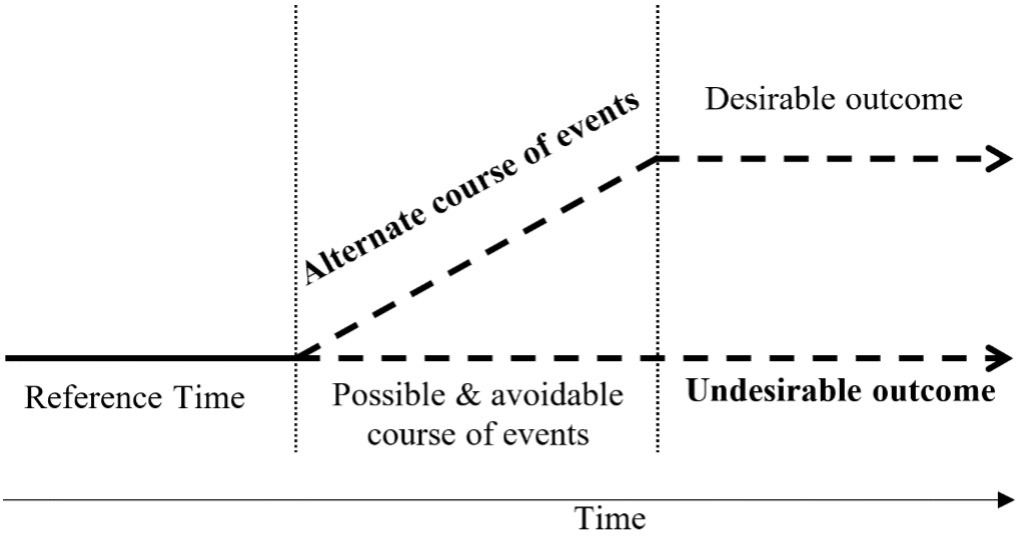
\includegraphics[width=.8\textwidth]{figures/fig1browne.jpg}
    \label{fig1}
\end{figure}

By \textsc{undesirable}, we refer to some event or entity that is evaluated as something that should be avoided. This evaluation is from the speaker's perspective on behalf of the person they are warning, and broadly relates to a negative outcome, whether due to an event, an event associated with an entity, or simply the coincidence of the subject and another entity. By \textsc{avoidable} we mean that an alternate course of action should be salient to the addressee, as in \REF{ex:bro1}, where the speaker overtly specifies the available course of action through an imperative clause `get down from there'.
\newpage
\ea 
\textnormal{\ili{Mudburra} (\ili{Ngumpin-Yapa})}\\
\gll Karu jurd wandi, bi=ngku linymurr ka-yinarra yali karndi=ma. \\
child {get\_down} fall[\textsc{imp}] \textsc{appr=2sg.ns} break be-\textsc{spec} that tree=\textsc{top} \\
\glt `Kid, get down from there [alternate course of events], (or else) that tree might break on you [undesirable outcome]!' [SD:DOS1-2017\_017-02:2674149\_2677841]\\
\label{ex:bro1}
\z

 The alternate course of events allowing the undesirable outcome to be avoided may be explicit, as above in \REF{ex:bro1} or implicit, as in \REF{ex:bro2}. We will refer to a clause which makes the alternate course of events explicit as \textsc{preemptive} clause, following \citet[265]{evans_current_1995}. However, the syntactic relation between the two clauses in \ili{Ngumpin-Yapa} languages is unclear (this is taken up in \sectref{subsubsec:clause}).

\ea 
\textnormal{\ili{Warlmanpa} (\ili{Ngumpin-Yapa})}\\
\gll Nga=nyanu-n=nga kuma-nma! \\
\textsc{appr=refl-2sg.s=appr} cut-\textsc{pot} \\
\glt `You might cut yourself!' $[$H\_K01-505B, DG, 38:14$]$ \\
\label{ex:bro2}
\z

 \citeauthor{lichtenberk_apprehensional_1995} makes a distinction between situations in which the eventuality may be avoided altogether, and where the effects of the eventuality may be mitigated \citep[297]{lichtenberk_apprehensional_1995}, though we have no clear data for the latter in these languages. As will be shown in the survey (\sectref{subsec:auslang}), only one Australian language (\ili{Martuthunira}) is known to grammatically distinguish these two functions. For the purposes of this paper, the alternate course of events may either avoid the event altogether, or mitigate the effects of the event (thus avoiding the undesirable outcome regardless).

Australian languages have a number of lexical and morphosyntactic strategies to convey apprehensional situations. Grammaticalised morphemes with apprehensional functions have been identified within verbal and nominal paradigms (i.e.\  morphological strategies); we also find grammaticalised multi-clausal constructions which convey apprehension (i.e.\  syntactic strategies).

In this chapter, we focus on investigating the degree to which apprehension has been grammaticalised in \ili{Ngumpin-Yapa} languages, a subgroup of the \ili{Pama-Nyungan} language family. We begin by first surveying apprehension cross-linguistically within Australia (\sectref{subsec:auslang}) and present a grammatical overview of \ili{Ngumpin-Yapa} languages (\sectref{subsec:NYlangs}), leading into a systematic account of apprehensional constructions in these languages. We discuss the various functions of the aversive case (relational, subordinating, and insubordinate functions signalling apprehension, \sectref{subsec:aversivecase}); the marking of complements of `fear' predicates (\sectref{subsec:complements}), as well the encoding of apprehension by a morpheme known as the auxiliary (\sectref{subsec:auxiliaries}). Finally, we consider the range of functions that sentences involving apprehensionals tend to serve in discourse, divided into directives and assertives (\sectref{sec:discourse}). 



\subsection{Apprehension in Australian languages}
\label{subsec:auslang}

In descriptions of Australian languages, apprehensional morphemes have been assigned a number of terminological labels, reflecting the lack of a unified approach to understanding these morphemes. \tabref{tab1-bro} exemplifies the wide array of glosses given to apprehensional morphemes in grammars of Australian languages.



\begin{table}

\caption{Sample of the various glosses given to apprehensional morphemes.}
\label{tab1-bro}
\begin{tabularx}{\textwidth}{lQlQ}
\lsptoprule
Language & Morpheme(s)                                        & Gloss             & Reference \\
\midrule
\ili{Djabugay}          & \textit{lan, -ndabi, -ndjabi  }          & `aversive'                 & \citep[268]{patz_djabugay_1991}                  \\
\tablevspace
\ili{Wangkajunga}       & \textit{-ngkamarra}                      & `avoidance'                & \citep[95, 290--291]{jones_grammar_2011}                  \\
\tablevspace
\ili{Kayardild}         & \textit{waalu-tha/-waal-i-ja  }       & `evitative'                & \citep[173--175]{evans_current_1995}                  \\
\tablevspace
\ili{Warumungu}         & \textit{-kajji}                          & `lest'                     & \citep[22--23]{simpson_warumungu_1982}                  \\
\tablevspace
\ili{Alyawarra}         & \textit{-ikitja}                         & `negative causative'       & \citep[69, 75--76]{yallop_alyawarra_1977}                  \\
\tablevspace
\ili{Walmajarri}        & \textit{-ngkamarra}                      & `projected reason'         & \citep[31]{hudson_core_1978}                  \\
\tablevspace
\ili{Mangarrayi}        & \textit{ba\d{l}aga}                          & `evocative/anticipatory' & \citep[146--147]{merlan_mangarayi_1989}                  \\
\tablevspace
\ili{Ngarinyman}        & \textit{ngaja}                           & `apprehensive'             & \citep{angeloschultzeberndt2016}                 \\
\tablevspace
\ili{Bilinarra}         & \textit{ngaja}                           & `admonitive'               & \citep[305]{meakins_grammar_2014}\\
\lspbottomrule
\end{tabularx}
\end{table}

Moreover, while many Australian languages appear to have some strategy for encoding apprehensional meanings, there has been very limited literature examining how these constructions vary across the continent.\footnote{\citet{gaby_expression_2017} presented an unpublished typology of apprehension in Australian languages.} A singular exception is \citeauthor{zester_semantics_2010}'s (2010) survey of apprehensional constructions in 8 \ili{Pama-Nyungan} languages and 4 non-Pama-Nyungan languages, which sought to compare the category of apprehension in Australian languages and \ili{English}.\footnote{The \ili{Pama-Nyungan} languages included in \citeauthor{zester_semantics_2010}'s study were: \ili{Yidiɲ}, \ili{Djabugay}, \ili{Pithanthathara}, \ili{Martuthunira}, \ili{Panyjima}. The non-Pama-Nyungan languages were \ili{Ndjébbana} (Arnhem), \ili{Gooniyandi} (\ili{Bunuban}), \ili{Wambaya} (\ili{Mirndi}) and \ili{Jingulu} (Mirndi). No \ili{Ngumpin-Yapa} languages were covered in \citeauthor{zester_semantics_2010}'s survey.} 

We categorise apprehensional morphemes into three distinct types based on morphosyntactic locus of exponence, described below:
\begin{enumerate}
\itemsep-0.2cm
    \item nominal case inflections;
    \item verbal mood inflections; and
    \item non-inflecting particles.
\end{enumerate}

\subsubsection{Nominal case suffixes}

\noindent Apprehensional suffixes in Australian languages occur within nominal paradigms, either as dedicated case suffixes or as a function of a case suffix not primarily apprehensional in nature. In \ili{Wargamay} (\ili{Dyirbalic}), for example, a locative suffix has a range of adjunct spatial functions, such as to mark location in space and time (`in', `at' `on', `near' etc.), accompaniment (`with') and circumstance (`while'). The \ili{Wargamay} locative case can also be used in apprehensional contexts, as in \REF{ex:bro3}, in which the locative suffix \textit{-nga} is used to indicate that the white man is something to be avoided.

\ea
\langinfo{Wargamay}{Dyirbalic} {\citealt[30]{dixon_wargamay_1981}} \\
\gll Ngayba bimbirigi waybala-\textbf{nga}. \\
\textsc{1sg.s} run.\textsc{perf} {white\_man-\textsc{\textbf{loc}}} \\
\glt `I'm running for fear of the white man.' 
\label{ex:bro3}
\z

 Other languages possess dedicated nominal suffixes for encoding apprehension. In the Australianist tradition, these are typically labelled `evitative' or `aversive' cases.\footnote{Henceforth we will generally refer to isomorphic case forms encoding apprehension as `aversive' cases and gloss them consistently as `\textsc{ave}'.} These suffixes encode that the referent of the case-marked phrase is to be avoided, often translated with some implicit eventuality associated with the referent, as in the \ili{Yidiɲ} example in \REF{ex:bro4}.

\ea 
\langinfo{Yidiɲ}{\ili{Yidinic}} {\citealt[262]{dixon_grammar_1977}} \\
\gll Jaja munubujun {nyinany \textnormal{/}} bama-\textbf{yida.} \\
child.\textsc{abs} inside:\textsc{still} sit:\textsc{pst} person-\textsc{\textbf{ave}} \\
\glt `The child still sat inside [the hut] for fear of [being seen by] the people.'
\label{ex:bro4}
\z

 In some languages, the dedicated case suffix is formally comprised of another case suffix as well as an apprehensional increment. In \ili{Pintupi}, for example, to form the `avoidance' case, the increment \textit{-marra} is added to a locative case form which marks accompaniment, animate goals, and animate locations \citep[57]{hansen_core_1978}. Examples \REF{ex:bro5} and \REF{ex:bro6} demonstrate the same stem \textit{mul̪ipuru} `one obscured by the shelter' in the locative (\textit{-ngka}) and avoidance cases (\textit{-ngkamarra}) respectively. This type of complex case formation is cross-linguistically common in Australia, and has been termed ``compound case'' \citep[256]{schweiger_compound_2000} or ``parasitic formation'' \citep[85--86]{matthews_morphology_1991}.



\ea
\langinfo{Pintupi}{\ili{Western Desert}} {\citealt[99]{hansen_core_1978}} \\
\gll Tjampitjin-ta=litju=lu watja{n̪}u, mul̪i-\textbf{puru-ngka}. \\
name-\textsc{loc=1du.excl.s=3sg.lct} said shelter\textbf{-\textsc{obsc-loc}}\\
\glt `We spoke to Tjampitjinpa who was obscured by the shelter.' 
\label{ex:bro5}
\z


\ea
\langinfo{Pintupi}{Western Desert} {\citealt[99]{hansen_core_1978}} \\
\gll Mul̪i-\textbf{puru-ngkamarra}=n̪a=lura {yarka-\emptyset} pitjangu. \\
shelter-\textbf{\textsc{obsc-ave}}=\textsc{1sg.s=3sg.ave} secret-\textsc{nom} went \\
\glt `To avoid that one who is obscured by the shelter, I kept myself hidden as I walked.'
\label{ex:bro6}
\z


\subsubsection{Verbal inflection}

Some Australian languages have a dedicated verbal inflection which signals apprehension. \ili{Martuthunira} (\ili{Ngayarta}, \ili{Pama-Nyungan}), for example, has a `lest' verb suffix which encodes apprehensional circumstances, exemplified in \REF{ex:bro7}.

\ea
\langinfo{Martuthunira}{Ngayarta}{\citealt[73]{dench_martuthunira_1995}} \\
\gll Nhiyu pawulu wangka-yangu puni-layi karla-ngku \textbf{kampa-wirri}, mir.ta waruul puni-nguru. \\
this child tell-\textsc{passp} go-\textsc{fut} fire-\textsc{eff} \textbf{burn-\textsc{appr}} not still go-\textsc{prs}\\
\glt `This child has been told to go lest he gets burnt by the fire, but he still hasn't gone.'
\label{ex:bro7}
\z

A less common locus of encoding apprehensional meanings across the Australian continent is that of a discontinuous inflection as in \ili{Nyangumarta} (\ili{Marrngu}, \ili{Pama-Nyungan}) \citep[165, 186--187]{sharp_nyangumarta_2004}, or a clitic as in another \ili{Marrngu} language, \ili{Mangarla} \citep[335]{agnew_core_2020} which takes predicates as its hosts, as shown in \REF{ex:bro8}. In the case of the latter, the status of the \textsc{antic}ipatory in \ili{Mangarla} as a clitic is affirmed by its co-occurrence with tense, aspect, mood (TAM) inflections other than the imperative and its (rare) encliticisation to nominal predicates.\footnote{The verb in \REF{ex:bro8} is glossed as an imperative, which expresses a wide range of functions in \ili{Mangarla} \citep[320]{agnew_core_2020}.}

\ea
\langinfo{Mangarla}{Marrngu}{\citealt[336]{agnew_core_2020}} \\
\gll Pantu warlu parra\textasciitilde parra kampa=nyjurruny=\textbf{kulu}. \\
\textsc{med} fire heat\textasciitilde \textsc{rdp} burn.\textsc{imp}=\textsc{1pl.incl.o=\textbf{antic}} \\
\glt `That fire is hot and might burn us.'
\label{ex:bro8}
\z

\largerpage
 There is variability across languages with respect to whether a given verbal inflection is a dedicated marker of apprehension or semantically less specific, e.g.\   whether it also has a general irrealis meaning denoting any possible and unrealised events which need not be negatively evaluated. For instance, \ili{Wargamay} has an `irrealis' verbal suffix which can be used in future, unreal and apprehensive contexts. The `irrealis' inflection is exemplified in \REF{ex:bro9}, where the event is not negatively evaluated, and in \REF{ex:bro10}, where it is.\footnote{Further examples are: the anticipatory inflection in \ili{Ngardi} (\ili{Ngumpin-Yapa}, \ili{Pama-Nyungan}; \cite{ennever_nominal_2018}), the subjunctive inflection in \ili{Yulparija} (\ili{Western Desert}, \ili{Pama-Nyungan}; \citep[39]{burridge_yulparija_1996} or the obligative and hypothetical inflections in \ili{Wangkajunga} (\ili{Western Desert}, \ili{Pama-Nyungan}; \cite[201--202]{jones_grammar_2011}). All of these inflections share a semantic basis that the speaker is conveying that the event is likely to occur. Undesirability does not seem to be encoded. In some languages, clausal negation affects possible interpretations, as in \ili{Mangarla} \citep[335--339]{agnew_core_2020}.}

\ea
\langinfo{Wargamay}{\ili{Dyirbalic}}{\citealt[54]{dixon_wargamay_1981}} \\
\gll Ngayba nga: \textbf{walama}. \\
\textsc{1sg.s} \textsc{neg} \textbf{ascend.\textsc{irr}} \\
\glt `I'm not climbing (anymore, because I'm tired).'
\label{ex:bro9}
\z

\ea
\langinfo{Wargamay}{\ili{Dyirbalic}}{\citealt[54]{dixon_wargamay_1981}} \\
\gll Ngaru {gilwalga \textnormal{/}} \textbf{ba:dima}. \\
\textsc{neg} kick.\textsc{neg.imp} \textbf{cry.\textsc{irr}} \\
\glt `Don't kick him, lest he cry / he might cry.'
\label{ex:bro10}
\z

In most Australian languages, where a verb suffix denotes an apprehensional meaning, the clause in which it occurs is usually either juxtaposed or subordinate to a main clause encoding a preemptive event, as in \REF{ex:bro11}, suggesting these verb inflections may be indicative of subordination.


\ea 
\langinfo{Yidiɲ}{\ili{Yidinic}} {\citealt[351]{dixon_grammar_1977}} \\
\gll Nyundu {gajidagan \textnormal{/}} giyara-nggu guba:-\textbf{nji}. \\
you:\textsc{erg} long\_way:\textsc{inch:vblsr:imp} stinging\_tree-\textsc{erg} burn-\textbf{\textsc{lest}} \\
\glt `You keep away, lest you get stung by the stinging tree!'
\label{ex:bro11}
\z

\subsubsection{Non-inflecting particles}

Some Australian languages have particles (often complementisers) which introduce a subordinate clause and place it in an apprehensional relation to the (preemptive) main clause. \citet{zester_semantics_2010} discusses two non-Pama-Nyungan languages in Australia's north exhibiting apprehensional complementisers: the \ili{Mirndi} languages \ili{Wambaya} \citep[210]{nordlinger_grammar_1998} and \ili{Jingulu} \citep{pensalfini_grammar_2003}. An example from \ili{Jingulu} is given in \REF{ex:bro12}, where the subordinate clause is headed by the evitative complementiser \textit{karningka} (glossed `\textsc{lest}').

\ea 
\langinfo{Jingulu}{\ili{Mirndi}} {\citealt[120]{pensalfini_grammar_2003}} \\
\gll Buba jimi-rni ila-mi jungkali marru-ngka-mbili \textbf{karningka}  buba-arndi ngunji-jiyimi marru. \\
firewood that(n)-\textsc{foc} put-\textsc{irr} far house-\textsc{all-loc} \textbf{\textsc{lest}} fire-\textsc{inst} burn-come house \\
\glt `Put the firewood down far from the house, lest the fire burn the house down.'
\label{ex:bro12}
\z

\subsubsection{No apprehensional morphemes}

Other languages may convey apprehension by the juxtaposition of a preemptive clause with a clause expressing a possibility, but without overt apprehensional morphology on the latter. In \ili{Warluwarra} (\ili{Ngarna}), there are no morphemes which could be clearly associated with apprehension. Instead, apprehension is derived via pragmatic enrichment in irrealis situations, particularly when juxtaposed with a preemptive clause, as in \REF{ex:bro13}.\footnote{Note that this is similar to languages which have an irrealis inflection or complementiser-like particles which are used in apprehensional constructions but do not encode specifically `apprehension'. In fact there may be no distinction between these two types. The distinction lies in how strongly the morphemes are associated with apprehension.} In this case, if the addressee smells the meat (preemptive), it mitigates the effects of it being rotten (for example, it results in them not eating it if it is rotten).

\ea
\langinfo{Warluwarra}{\ili{Ngarna}} {\citealt[234]{breen_description_1970}} \\
\gll Jatjunma jinja {karlaanha \textnormal{/}} warrɣa ngarlatha jiwa. \\
smell.\textsc{imp} that[\textsc{acc}] meat[\textsc{acc}] rotten maybe it \\
\glt `Smell that meat; it might be rotten.'
\label{ex:bro13}
\z

 \ili{Ngumpin-Yapa} languages present an opportunity to refine cross-linguistic generalisations regarding apprehensional constructions, particularly in the Australian context. Firstly, most \ili{Ngumpin-Yapa} languages exhibit both a nominal case suffix and a particle-like auxiliary to signal apprehension, unlike any other language surveyed in Australia. Additionally, \ili{Ngumpin-Yapa} languages, despite being a close-knit group of languages, show a very interesting diversity in the expression of complements of `fear' predicates and apprehensional marking in general.

\subsection{Ngumpin-Yapa languages}
\label{subsec:NYlangs}

This survey focuses on nine languages of the \ili{Ngumpin-Yapa} subgroup, a subgroup within the widespread \ili{Pama-Nyungan} family in Australia. The languages for which data is discussed in this paper are: \ili{Walmajarri}, \ili{Jaru}, \ili{Ngardi}, \ili{Gurindji}, \ili{Wanyjirra}, \ili{Bilinarra}, \ili{Mudburra}, \ili{Warlmanpa} and \ili{Warlpiri}. Our current understanding of their relative cladistic relationships within the \ili{Ngumpin-Yapa} subgroup is represented in \figref{fig2}. The areal distribution of \ili{Ngumpin-Yapa} languages across northwestern Australia is shown in \figref{fig3}.


\begin{figure}[p]
\small
\fittable{
\begin{forest}for tree={grow'=east,draw,minimum width=2.2cm}, forked edges,  where n children=0{fill=gray!20}{}
[\ili{Ngumpin-Yapa}
    [Ngumpin
        [Western Ngumpin
            [\textbf{Walmajarri}]
            [\textbf{Ngardi}]
            [\textbf{Jaru}]
            [\textbf{Wanyjirra}]
        ]
        [Eastern Ngumpin
            [Victoria River
                [\textbf{Gurindji}]
                [\ili{Malngin}]
                [\textbf{Bilinarra}]
                [\ili{Ngarinyman}]
            ]
            [Far Eastern
                [\ili{Karranga}]
                [\textbf{Mudburra}]
            ]
        ]
    ]
    [Yapa
        [\textbf{Warlpiri}]
        [\textbf{Warlmanpa}]
    ]
]
\end{forest}
}
    \caption{Phylogeny of the Ngumpin-Yapa subgroup. Languages included in this study are emphasised. Adapted from \citet[791]{mcconvell_loanwords_2009}}
%     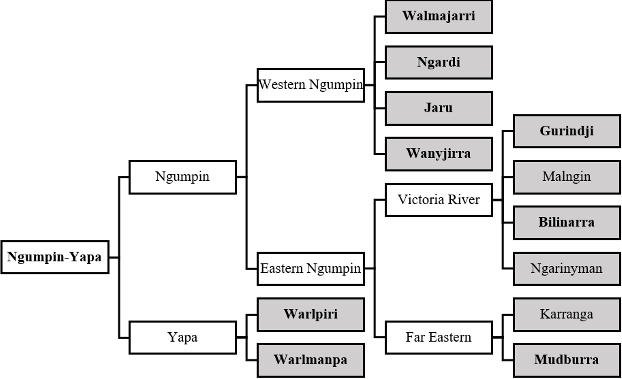
\includegraphics[width=1\textwidth]{figures/fig2browne.png}
    \label{fig2}
\end{figure}

\begin{figure}[p]
    \caption{Map of relative locations of Ngumpin-Yapa languages across northern Australia (adapted from \cite{meakins_possessor_2017}; cartographer: Brenda Thornley).}
    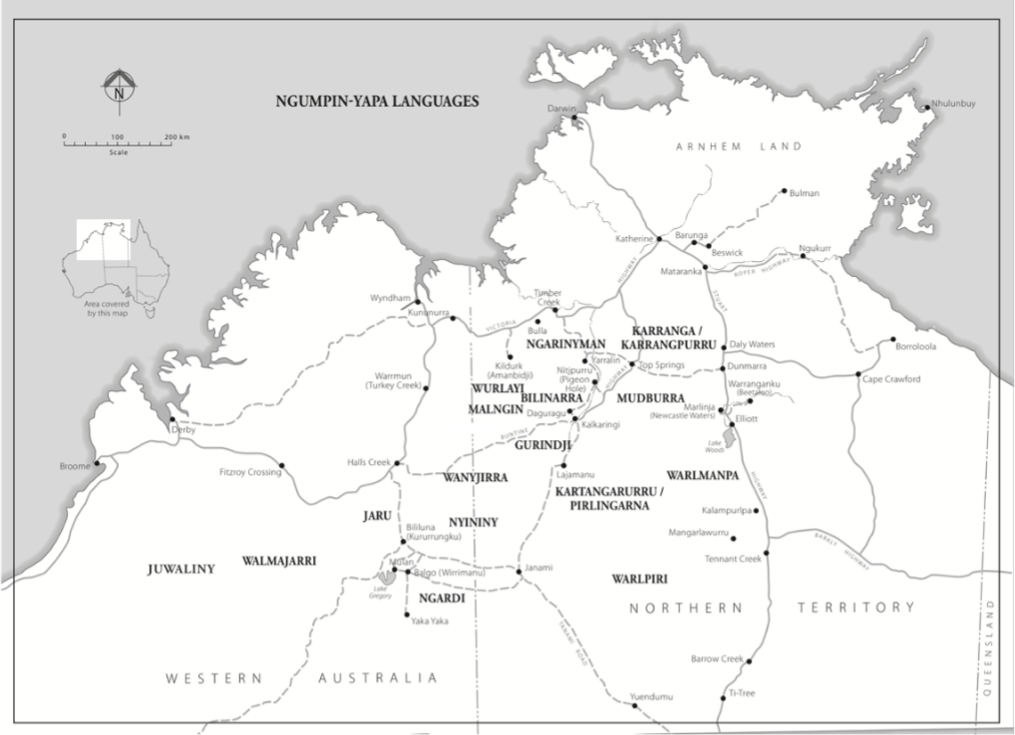
\includegraphics[width=.9\textwidth]{figures/fig3browne.png}
    \label{fig3}
\end{figure}


Evidence for the unity of the Ngumpin and Yapa subgroups, and for their position within the \ili{Nyungic} subgroup, is provided by \citet{laughren_ngumpin-yapa_2004}, while evidence adduced from pylogenetic studies is provided by \citet{bowern_computational_2012} on the basis of lexical data, and by \citet{macklin-cordes_high-definition_2015} on the basis of phonotactic data. In this section, we briefly detail some of the relevant morphosyntactic characteristics of these languages. 

A working orthography of all the languages used in this survey is presented in \tabref{tab2-bro}. The only phoneme not shared across the subgroup is a retroflex flap which is only fully phonemicised in certain dialects of \ili{Warlpiri} and is otherwise an allophone of the retroflex stop (Western \ili{Warlpiri}) or an allophone of the retroflex continuant (glide) phoneme (\ili{Ngardi} and \ili{Jaru}). As for stops, voicing is not distinctive in the languages under discussion. Across the \ili{Ngumpin-Yapa} languages there are three orthographies in use which largely differ by the representation of stops.\footnote {p \textasciitilde t \textasciitilde k: \ili{Gurindji}, \ili{Warlpiri}, \ili{Ngardi}, \ili{Warlmanpa} \\
b \textasciitilde d \textasciitilde k: \ili{Mudburra} \\
b \textasciitilde d \textasciitilde g: \ili{Bilinarra}, \ili{Ngarinyman}, \ili{Wanyjirra}} We retain the orthography from source materials in examples. 


\begin{table}

\caption{Maximal Ngumpin-Yapa consonant phoneme inventory (orthographic forms given in brackets where they differ from the expected IPA symbol)}
\label{tab2-bro}
\begin{tabular}{llllll}
\lsptoprule
           & \multicolumn{2}{c}{{Peripheral}} & \multicolumn{2}{c}{{Apical}}    & Laminal \\
           & Bilabial    & Velar   & Alveolar & Retroflex & Palatal \\ \midrule
Stop       & p/b                & k/g            & t/d              & \textrtailt \hspace{0.1cm} <rt/rd>          & c \hspace{0.1cm} <j>            \\
Nasal      & m                    & \ng \hspace{0.1cm} <ng>             & n                 & \textrtailn \hspace{0.1cm} <rn>               & \textltailn \hspace{0.1cm} <ny>             \\
Lateral    &                      &                  & l                 & \textrtaill \hspace{0.1cm} <rl>               & \textturny \hspace{0.1cm} <ly>           \\
Flap/Trill &                      &                  & r \hspace{0.1cm} <rr>            & \textrtailr \hspace{0.1cm} <rd>               &                  \\
Glide      & w                    &                  &                   & \textturnrrtail \hspace{0.1cm} <r>                & j \hspace{0.1cm} <y>            \\
\lspbottomrule
\end{tabular}
\end{table}

All \ili{Ngumpin-Yapa} languages have a three-way distinction in vowel quality with most languages generally described as having a marginal length contrast with a low functional load (\tabref{tab3-bro}).

\begin{table}

\caption{Ngumpin-Yapa vowel inventory}
\label{tab3-bro}
\begin{tabular}{lll}
\lsptoprule
          & Front & Back \\ \midrule
High      & i, (ii)        & u, (uu)       \\
Low       & a, (aa)        &               \\ 
\lspbottomrule
\end{tabular}
\end{table}

\ili{Ngumpin-Yapa} languages are agglutinating and purely suffixing. Core arguments are case-marked and are also cross-referenced by bound pronominal enclitics which encode person, number and case features. These languages all demonstrate the properties of non-configurationality as described for \ili{Warlpiri} \citep{hale_warlpiri_1983}, including: free word order, discontinuous phrase structure and frequent ellipsis of nominals. All \ili{Ngumpin-Yapa} languages share the property that the pronominal clitics generally occupy second position of the clause, so-called Wackernagel's position \citep{wackernagel_uber_1892}. Other features of these clitics vary considerably across the subgroup -- both with respect to the range of grammatical relations that bound pronouns may cross-reference, and the types of clausal elements to which they may attach.

One type of host for the pronominal clitics are termed \textit{auxiliary bases}. These are otherwise uninflecting particles which obligatorily host the pronominal clitics. The semantics of the auxiliary base varies considerably across languages. In some cases, the auxiliary base is essentially a meaningless host for the pronominal enclitics and has been termed ``catalyst'' by some authors, for example \textit{ba} in \ili{Mudburra} \citep[68--69]{capell_new_1956}, \textit{ngu} in \ili{Gurindji} \citep{mcconvell_functions_1996}, and \textit{nga} in \ili{Ngarinyman} \citep[30]{jones_ngarinyman_2019}. In some \ili{Ngumpin-Yapa} languages, there is a small inventory of semantically meaningful auxiliaries (or ``modal particles''), which contribute tense, aspect, or mood information to the clause. For example, the auxiliaries in \ili{Warlpiri} include \textit{lpa} `imperfective' and \textit{ka} `present' \citep{laughren_revised_2013}, which combine with verb inflections to encode fine-grained TAM distinctions.\footnote{Western \ili{Warlpiri} has a future verb inflection in addition to the auxiliaries.} 

In nearly all \ili{Ngumpin-Yapa} languages, lexemes of certain other grammatical categories also attract the pronominal enclitics (in lieu of an auxiliary base in the given construction), including complementisers, interrogatives as well as imperative-inflected verbs. In languages without a catalyst auxiliary, such as \ili{Ngardi}, in the absence of any of these more typical hosts, the bound pronouns encliticise to the first phonological word (or in some cases, the first phrase) \citep[310--313]{ennever_grammar_2021}.

These bound pronominals pattern primarily according to a nominative-accusative system, in which A and S are encoded by a subject series, and O is encoded by an object series. For many of the languages surveyed, there is syncretism between the object (\textsc{o})  and oblique (\textsc{obl}) series in all subject/number combinations except \textsc{3sg}, leading to the convention of labelling these forms as either \textsc{o} `object/oblique', or \textsc{ns} `non-subject'. In nearly all of the Ngumpin languages, nominals in certain other (traditionally semantic) cases such as the locative, allative and ablative can also be cross-referenced by bound pronominals (which, if distinct from the oblique, are labelled \textsc{lct} `locational' here), whereas this is not permitted in either of the Yapa languages. Language-specific systems are given in \tabref{tab4-bro}. \ili{Ngumpin-Yapa} languages do not utilise the bound pronominal system for aversive case-marked adjuncts (\sectref{subsec:aversivecase}), but do for complements of `fear' predicates (\sectref{subsec:complements}).


\begin{table}

\caption{Relationship between case marking and the cross-referencing bound pronouns.}
\label{tab4-bro}
\begin{tabularx}{\textwidth}{lX ll @{\quad} llllll}
\lsptoprule
 & & \multicolumn{2}{c}{ {Subject}} & \multicolumn{5}{c}{ {Non-subject}} &  \\
%  \cmidrule(lr){3-4}\cmidrule(lr){5-9}
 & {Case} & {\textsc{erg}} & {\textsc{abs}} & {\textsc{abs}} & {\textsc{dat}} & {\textsc{loc}} & {\textsc{all}} & {\textsc{abl}}\footnote{We use the case label \textit{ablative} here, however \textit{elative} is used for some languages.} &  \\
 \midrule
 & \ili{Warlpiri} & \cellcolor[HTML]{8D8D8D}S & \cellcolor[HTML]{8D8D8D}S & \cellcolor[HTML]{9B9B9B}O & \cellcolor[HTML]{C0C0C0}\textsc{obl} & --- & --- & --- &  \\
\multirow{-2}{15mm}{Yapa} & \ili{Warlmanpa} & \cellcolor[HTML]{8D8D8D}S & \cellcolor[HTML]{8D8D8D}S & \cellcolor[HTML]{9B9B9B}O & \cellcolor[HTML]{C0C0C0}\textsc{obl} & --- & --- & --- &  \\

\tablevspace

& \ili{Bilinarra} & \cellcolor[HTML]{8D8D8D}S & \cellcolor[HTML]{8D8D8D}S & \cellcolor[HTML]{9B9B9B}O & \cellcolor[HTML]{C0C0C0}\textsc{obl} & --- & --- & --- &  \\
 & \ili{Gurindji}\footnote{This follows \citeauthor{mcconvell_functions_1996}'s (\citeyear[84]{mcconvell_functions_1996}) analysis of bound pronouns in \ili{Gurindji}, where ``affected locations $\ldots$ are cross-referenced by clitics, unlike other locations, and in a way distinct from either S, O, or IO clitics.''} & \cellcolor[HTML]{8D8D8D}S & \cellcolor[HTML]{8D8D8D}S & \cellcolor[HTML]{9B9B9B}O & \cellcolor[HTML]{C0C0C0}\textsc{obl} & \cellcolor[HTML]{D9D6D6}\textsc{lct} & \cellcolor[HTML]{D9D6D6}\textsc{lct} & \cellcolor[HTML]{D9D6D6}\textsc{lct} &  \\
 & \ili{Mudburra} & \cellcolor[HTML]{8D8D8D}S & \cellcolor[HTML]{8D8D8D}S & \cellcolor[HTML]{9B9B9B}O & \cellcolor[HTML]{C0C0C0}\textsc{obl} & \cellcolor[HTML]{C0C0C0}\textsc{obl} & \cellcolor[HTML]{C0C0C0}\textsc{obl} & --- &  \\
\multirow{-4}{15mm}{Eastern\newline Ngumpin  } & \ili{Wanyjirra} & \cellcolor[HTML]{8D8D8D}S & \cellcolor[HTML]{8D8D8D}S & \cellcolor[HTML]{9B9B9B}O & \cellcolor[HTML]{C0C0C0}\textsc{obl} & \cellcolor[HTML]{C0C0C0}\textsc{obl} & \cellcolor[HTML]{C0C0C0}\textsc{obl} & \cellcolor[HTML]{C0C0C0}\textsc{obl} &  \\

\tablevspace

 & \ili{Jaru} & \cellcolor[HTML]{8D8D8D}S & \cellcolor[HTML]{8D8D8D}S & \cellcolor[HTML]{9B9B9B}O & \cellcolor[HTML]{C0C0C0}\textsc{obl} & \cellcolor[HTML]{D9D6D6}\textsc{lct} & \cellcolor[HTML]{D9D6D6}\textsc{lct} & \cellcolor[HTML]{D9D6D6}\textsc{lct} &  \\
 & \ili{Ngardi} & \cellcolor[HTML]{8D8D8D}S & \cellcolor[HTML]{8D8D8D}S & \cellcolor[HTML]{9B9B9B}O & \cellcolor[HTML]{C0C0C0}\textsc{obl} & \cellcolor[HTML]{D9D6D6}\textsc{lct} & \cellcolor[HTML]{D9D6D6}\textsc{lct} & --- &  \\
\multirow{-3}{15mm}{Western\newline Ngumpin  } & \ili{Walmajarri} & \cellcolor[HTML]{8D8D8D}S & \cellcolor[HTML]{8D8D8D}S & \cellcolor[HTML]{9B9B9B}O & \cellcolor[HTML]{C0C0C0}\textsc{obl} & \cellcolor[HTML]{D9D6D6}\textsc{acs} & --- & --- &  \\
\lspbottomrule
\end{tabularx}
  %
\end{table}

All \ili{Ngumpin-Yapa} languages exhibit extensive case marking. Nominals bear no overt case marking in the S and O function, and bear overt ergative case marking in the A function (in accordance with an ergative-absolutive case-marking pattern). While free pronouns in \ili{Warlpiri}, \ili{Ngardi}, \ili{Jaru}, \ili{Walmajarri}, and Eastern \ili{Mudburra} exhibit ergative-absolutive marking like other nominals, in \ili{Wanyjirra}, \ili{Gurindji}, \ili{Bilinarra}, Western \ili{Mudburra} and \ili{Warlmanpa}, free pronouns are invariably unmarked in all three core functions.

All \ili{Ngumpin-Yapa} languages possess two morphosyntactically distinct parts of speech with verbal semantics: inflecting verbs and coverbs. Inflecting verbs are a closed class of inflecting words (from around thirty to over a hundred) which bear tense/aspect/mood inflection; however the languages vary considerably in terms of the number and type of features encoded by verbal inflections. Variation is found, for example, in the distinctions made for past time reference (with a particularly differentiated system in \ili{Jaru} and \ili{Ngardi}), the presence of associated motion markers (\ili{Mudburra}, \ili{Ngardi}, \ili{Warlpiri}, \ili{Warlmanpa}), the presence of directional suffixes which can be cumulatively realised with another feature (\ili{Ngardi}, \ili{Warlpiri}), and patterns of reduplication (with a particularly complex system in \ili{Mudburra}). An inflecting verb may constitute a simple predicate on its own, or it may act as a light verb in a complex predicate along with a coverb (also called a ``preverb''; see \citealt{Osgarby_complexpred}).

\ili{Ngumpin-Yapa} languages exhibit both finite and non-finite subordination. The latter typically involves a non-finite verb form or a coverb bearing complementiser case suffixes, expressing the relative time and, in some cases, control properties of the subordinate clause \citep{simpson_control_1983}. Finite subordination is achieved by the use of a complementiser particle within the finite subordinate clause. Such clauses may have both temporal (T-relative) or anaphoric (NP-relative) functions; however multiple interpretations for the relationship between clauses are usually possible \citep{hale_adjoined_1976}.




\section{Morphosyntax of apprehension in Ngumpin-Yapa languages}
\label{sec:morphosyntax}

The complete inventory of grammatical markers of apprehension in \ili{Ngumpin-Yapa} languages is presented in \tabref{tab4-bro} and visually represented in \figref{fig4}. Three loci of grammaticalised apprehensional marking have been identified. The first is what will be termed an \textit{aversive case}, a dedicated nominal case suffix, which can mark a nominal referent as something which is feared, or a non-finite clause which denotes an undesired outcome. The second is the idiosyncratic marking of complements of `fear' predicates. These are treated as a grammaticalised form of apprehensional marking since their marking is idiosyncratic but shows some relationship to the grammar of apprehension elsewhere in the languages. The third is an auxiliary (although in some languages these auxiliaries are more complementiser- or particle-like) which indicates that the event referred to by the finite clause is undesired. While most languages have all three constructions available, \ili{Bilinarra} and \ili{Jaru} lack an aversive case suffix.





The aversive case is discussed in \sectref{subsec:aversivecase}, first exemplifying its relational function (\sectref{subsubsec:relational}), then its subordinate function (\sectref{subsubsec:subordinating}), before discussing the issues in accurately distinguishing the two functions (\sectref{subsubsec:clause}). Furthermore, in some languages these cases exhibit insubordinate functions (\sectref{subsubsec:insubordinate}). `Fear' complementation is discussed in \sectref{subsec:complements}: strategies include the locative case (\sectref{subsubsec:locative}), the dative case (\sectref{subsubsec:dative}), as well as the aversive (\sectref{subsubsec:aversive}). These variable case-marking patterns are summarised in \tabref{tab5-bro}. Finally, in \sectref{subsec:auxiliaries} we analyse the auxiliaries, discussing their syntactic properties in \sectref{subsubsec:syntacticstatus} and whether they are dedicated to encoding apprehension or not in \sectref{subsubsec:functionalstatus}.


\begin{figure}[t]
    \caption{Geographical distribution of dedicated apprehensional markers in Ngumpin-Yapa languages.}
    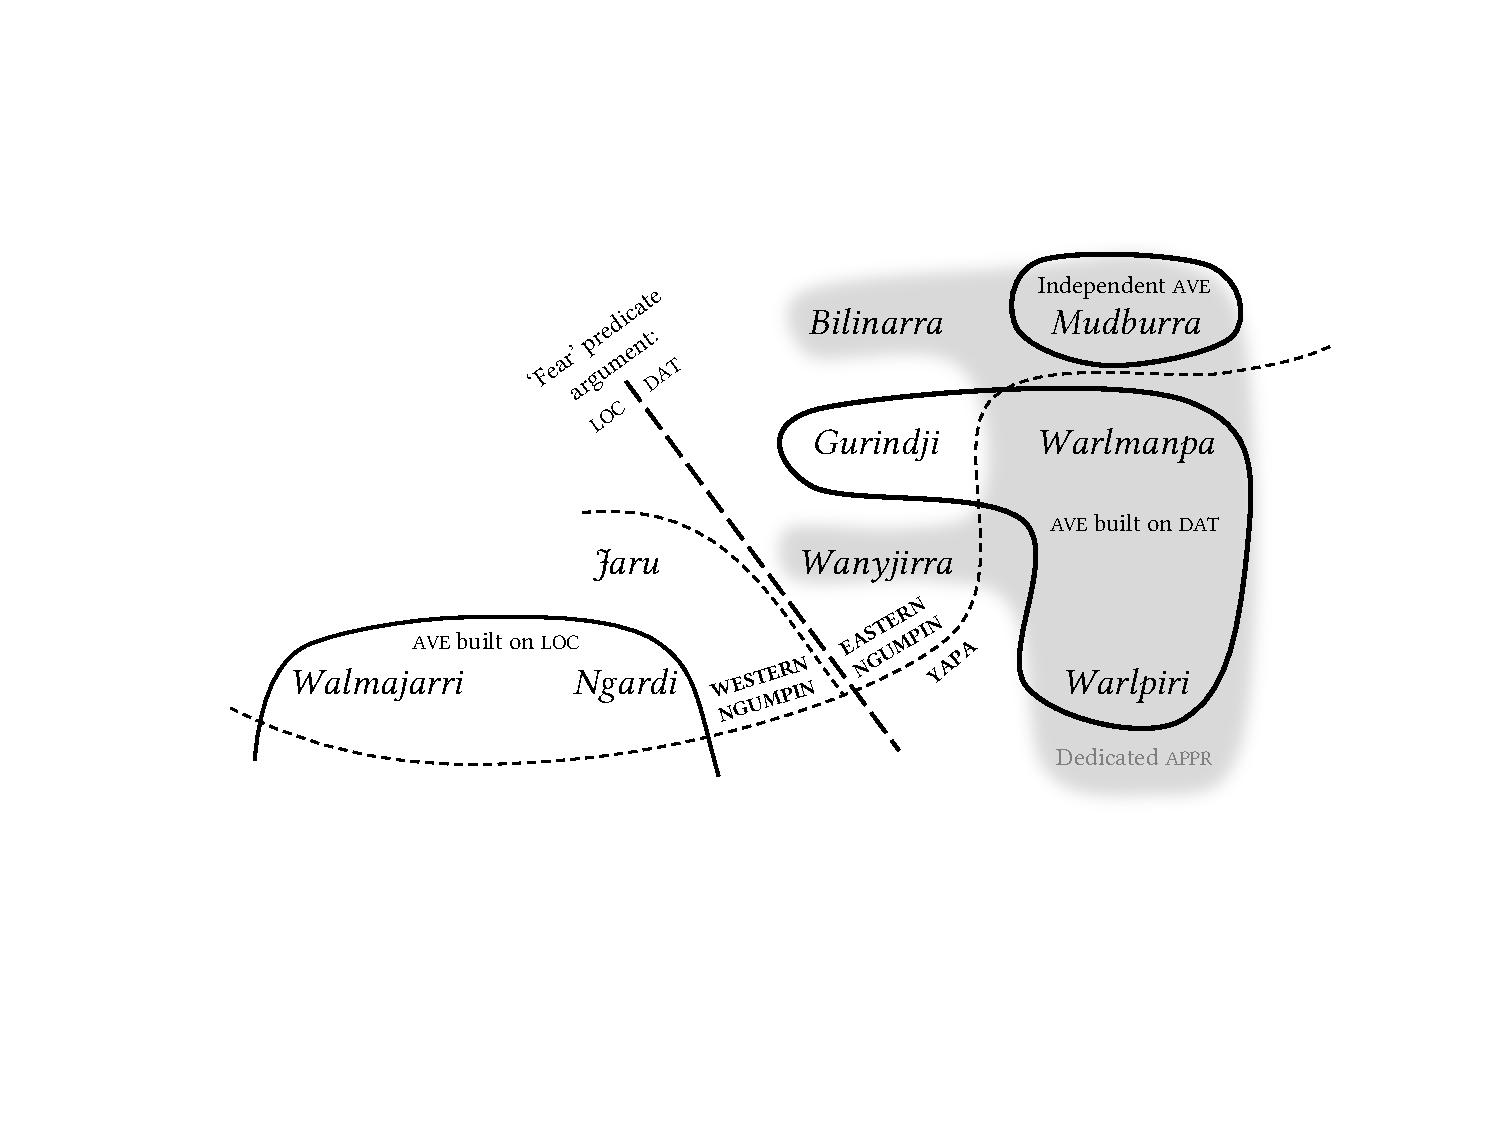
\includegraphics[width=1\textwidth]{figures/fig4browne.pdf}
    \label{fig4}
\end{figure}


\begin{table}
\caption{Overview of morphemes used to signal apprehension in Ngumpin-Yapa languages.}
\label{tab5-bro}
\begin{tabularx}{\textwidth}{p{1.5cm}lQQQ}
\lsptoprule
 & {{Language}} & {{Case in  aversive\newline function  }} & {{Case on `fear'\newline complement  }} & {{Auxiliary}\footnote{Note that in the \textit{auxiliary} column we have retained the authors' glossing, however elsewhere we have glossed these auxiliaries \textsc{appr} in order to allow ready comparison across languages. The \textit{-Ca} forms in the \textit{aversive function} column represent forms which exhibit extensive allomorphy conditioned by the preceding segment and the syllable or mora count of the stem.}} \\ \midrule
Yapa & \ili{Warlpiri} & \textit{-kujaku} \textsc{ave} & \textsc{dat}, \textsc{ave} & \textit{kalaka/kajika}\newline \textsc{pot}   \\
\tablevspace
 & \ili{Warlmanpa} & \textit{-kuma} \textsc{ave} & \textsc{dat} & \textit{kala(ka)} \textsc{appr}\newline \textit{nga=\ldots=nga}\newline \textsc{fut}=\ldots=\textsc{pot}   \\
 \midrule
Eastern\newline Ngumpin   & \ili{Bilinarra} & \textit{-ngka, -la, -Ca}\newline \textsc{loc}   & \textsc{dat} & \textit{ngaja} \textsc{adm} \\
\tablevspace
 & \ili{Gurindji} & \textit{-kumpalng},\newline \textit{-wumpalng} \textsc{ave}   & \textsc{dat} & \textit{ngaja} \textsc{adm} \\
\tablevspace
 & \ili{Mudburra} & \textit{-wirri} \textsc{ave} & \textsc{dat}, \textsc{ave} (rare) & \textit{bi(ya)} \textsc{appr} \\
\tablevspace
 & \ili{Wanyjirra} & \textit{-kunyja},\newline \textit{-wunyja} \textsc{com}    & \textsc{dat} & \textit{ngarra} \textsc{adm} \\

 \midrule
Western\newline Ngumpin & \ili{Jaru} & \textit{-ngka, -la, -Ca}\newline \textsc{loc}   & \textsc{loc} & \textit{ngarra}\newline `possible'   \\
\tablevspace
 & \ili{Ngardi} & \textit{-Camarra} \textsc{ave} & \textsc{loc}, \textsc{ave} & \textit{ngarda} \textsc{hyp} \\
\tablevspace
 & \ili{Walmajarri} & \textit{-Camarra,}\newline \textit{-karrarla} \textsc{ave}   & \textsc{loc}, \textsc{ave} (rare) & \textit{nga-rta} \textsc{mr1-dub}\newline  \textit{pa-rta} \textsc{mr2-dub}   \\
\lspbottomrule
\end{tabularx}
\end{table}



\subsection{Aversive case}
\label{subsec:aversivecase}

Six \ili{Ngumpin-Yapa} languages possess an aversive case suffix that can be classified as a dedicated apprehensional morpheme. Three languages lack a dedicated case suffix for expressing apprehension, and instead allow apprehensional meanings to be encoded by a polyfunctional case such as locative or comitative. In \figref{fig4} we distinguish between aversive case suffixes that are formally independent of other suffixes (\ili{Mudburra}), those built on the dative case suffix (\ili{Gurindji}, \ili{Warlpiri}, \ili{Warlmanpa}), and those built on the locative case suffix (\ili{Walmajarri}, \ili{Ngardi}). \ili{Warlpiri}, \ili{Warlmanpa} (Yapa) and \ili{Gurindji} (Eastern Ngumpin) all have aversive case forms which seem to be comprised of the dative case suffix \textit{-ku} \textasciitilde \textit{-wu} plus an increment, together marking the aversive case. 

\largerpage
Two Western Ngumpin languages (\ili{Walmajarri} and \ili{Ngardi}) possess aversive suffixes formally built on a locative case allomorph \textit{-Ca} + an increment \textit{-marra}. This case formation (\textsc{loc} + \textit{marra}) is widespread in the \ili{Western Desert} languages to the south of \ili{Walmajarri} and \ili{Ngardi}, for example \ili{Kukatja} and \ili{Wangkajunga}. A further variant is \textit{-karrarla} in \ili{Walmajarri}. Interestingly, a locative formative \textit{-rla} is still involved in \textit{-karrarla} but as the right-most constituent, with a base \textit{-karra}. An example is provided in \REF{ex:bro14}.

\ea
\langinfo{Walmajarri}{Western Ngumpin} {\citealt{richards_interactive_2012}} \\
\gll Kiwiri ma=rnalu jart-kuji-lany mimi-\textbf{karrarla.} \\
wood \textsc{mr1=1pl.excl.s} burn-\textsc{caus-cust} sick-\textbf{\textsc{ave}} \\
\glt `We would burn the \textit{kiwiri} wood to keep away sickness.' 
\label{ex:bro14}
\z

\noindent Like many other case suffixes in \ili{Ngumpin-Yapa} languages, the aversive case can either mark a participant in a particular semantic relation to the clausal predicate (\sectref{subsubsec:relational}) or it may serve as a subordinating case suffix (\sectref{subsubsec:subordinating}). These functions have been termed \textit{relational} and \textit{complementiser} functions by \citet{dench_multiple_1988} -- although the two are not always easily distinguished (\sectref{subsubsec:clause}). Additionally, aversive cases may appear in insubordinate constructions (\sectref{subsubsec:insubordinate}). These constructions lack a main clause predicate and instead the implied event associated with the participant marked by the case is insubordinated, i.e.\  appears in a main clause function (see \cite{evans_insubordination_2016}). In all cases in the corpora that we are aware of, the aversive case is used to indicate an entity or situation which is to be avoided, rather than indicating a situation to be mitigated.

\subsubsection{Relational function}
\label{subsubsec:relational}
%\largerpage[2]

Aversive case-marked NPs in all main clause types introduce a referent to be feared/negatively evaluated; and prototypically provide a justification for the action described by the remainder of the clause. Examples include (\ref{ex:bro15}) to (\ref{ex:bro17}).\footnote{In \ili{Ngumpin-Yapa} languages (and indeed other Australian languages with complex predicates), there is not always a straightforward link between the glosses of predicates and the given translation, as is the case in (\ref{ex:bro15}) where the inflecting verb is glossed `fall' yet this does not form part of the translation. It is often the case that the coverb bears the lexical information, and the inflecting verb essentially only bears grammatical (tense, mood, and aspect) information.}  


\ea
\textnormal{\ili{Mudburra} (Eastern Ngumpin)\footnote{\ili{Mudburra}, \ili{Ngardi}, and \ili{Warlmanpa} data come directly from corpora. The reference format of \ili{Mudburra} and \ili{Ngardi} is: 
Speaker initials: Audio code: Timestamp. 
The reference format of the \ili{Warlmanpa} data is: 
Audio code: Speaker initials: Timestamp.}}\\
\gll Yurrub wandi \textbf{ngarrambalyangka-wirri}.\\
hide fall.\textsc{imp} \textbf{police-\textsc{ave}}\\
\glt `Hide, for fear of the police!'%\footnote{In \ili{Ngumpin-Yapa} languages (and indeed other Australian languages with complex predi-cates), there is not always a straightforward link between the glosses of predicates and the given translation, as is the case in this example where the inflecting verb is glossed `fall' yet this does not form part of the translation. It is often the case that the coverb bears the lexical information, and the inflecting verb essentially only bears grammatical (tense, mood, and aspect) information.} 
\small{$[$MSD: AHA1-2016\_027-03: 1708833\_1711002$]$}
\label{ex:bro15}
\z

\ea
\textnormal{\ili{Ngardi} (Western Ngumpin)}\\
\gll Wakurra=rna wirriri ya-ni \textbf{mula-ngkamarra} \textbf{ngantany-jamarra.} \\
\textsc{neg=1sg.s} back go-\textsc{pst} \textbf{this-\textsc{ave}} \textbf{man-\textsc{ave}} \\
\glt `I didn't go back for fear of this man.' $[$PSM: TEN1-2017\_008-02: 938110\_946191$]$
\label{ex:bro16}
\z

\ea
\langinfo{Walmajarri}{Western Ngumpin} {\citealt{richards_interactive_2012}} 
\gll \textbf{Jilngin-tamarra} ma=rna kaniny\textasciitilde kaniny yuka-lku. \\
\textbf{dew-\textsc{ave}} \textsc{mr1=1sg.s} inside\textasciitilde \textsc{rdp} lie-\textsc{pot} \\
\glt `I'll sleep inside on account of the dew.' 
\label{ex:bro17}
\z

 In some languages, such as \ili{Jaru} (Western Ngumpin), the locative case can encode apprehension independent of a `fear' predicate as in \REF{ex:bro18}. Further, in \ili{Warlpiri} and \ili{Bilinarra}, the locative-marked nominal can comprise the entire utterance, as in \REF{ex:bro19}--\REF{ex:bro20}. Similarly, the comitative case (which prototypically encodes accompaniment) has an additional apprehensional function in \ili{Wanyjirra}, as in \REF{ex:bro21}.

\ea
\langinfo{Jaru}{Western Ngumpin} {\citealt[58]{tsunoda_djaru_1981}} \\
\gll Wanyja-rra gardiya-\textbf{la}! \\
leave-\textsc{imp} white\_man-\textbf{\textsc{loc}} \\
\glt `Leave (it) for fear of the white man (if you touch it, he might get angry).' 
\label{ex:bro18}
\z

\ea
\langinfo{Bilinarra}{Eastern Ngumpin} {\citealt[129]{meakins_grammar_2014}} \\
\gll Gawayi! Gurrurij-\textbf{ja}! \\
come\_here car-\textbf{\textsc{loc}}\\
\glt `Come here! Look out---car!'
\label{ex:bro19}
\z

\ea
\langinfo{Warlpiri}{Yapa}{Mary Laughren, p.c.} \\
\gll Warlu-\textbf{ngka}! \\
fire-\textbf{\textsc{loc}} \\
\glt `Look out for the fire!'
\label{ex:bro20}
\z

\ea
\langinfo{Wanyjirra}{Eastern Ngumpin} {\citealt[200]{senge_grammar_2015}} \\
\gll Ngu=rna=yanunggula wulaj garriny-ana yalu-\textbf{wunyja} garaj-\textbf{guja} ngaringga-\textbf{wuja}. \\
\textsc{real=1min.s=3aug.lct} hide stay-\textsc{prs} \textsc{dist2-\textbf{com}} human-\textbf{\textsc{com}} woman-\textbf{\textsc{com}} \\
\glt `I hide from that man and woman.'
\label{ex:bro21}
\z

 Aversive-marked NPs generally only have adjunct status in all \ili{Ngumpin-Yapa} languages, and as such they are never cross-referenced in the bound pronoun.\footnote{See the \ili{Walmajarri} example in \sectref{subsubsec:aversive} as an isolated exception.} This will be contrasted with complements of `fear' predicates in the dative and locative cases which are treated as clausal arguments (\sectref{subsec:complements}).

\subsubsection{Subordinating function}
\label{subsubsec:subordinating}

Aversive cases can also mark non-finite subordinate `lest' clauses, as in \REF{ex:bro22}.

\ea 
\textnormal{\ili{Warlmanpa} (Yapa)} \\
\gll Pingka pa-nka \textbf{wa-nja-kuma}. \\
slowly go-\textsc{imp} \textbf{fall-\textsc{inf-ave}} \\
\glt `Go slowly lest you fall.' $[$H\_K01-505B: DG, 43:43$]$
\label{ex:bro22}
\z

However, they are not necessarily dedicated apprehensional markers, and may more broadly mark undesirable events \REF{ex:bro23}, or events without a clear preemptive action \REF{ex:bro24}; or in the case of \ili{Warlpiri}, even impossible (yet desired) events \REF{ex:bro25}.


\ea
\langinfo{Warlpiri}{Yapa} {\citealt[53]{laughren_expressing_2015}} \\
\gll Pirtiri-ma-ni ka \textbf{ya-ninja-kujaku} janjanypa-rlu. \\
pester-\textsc{caus-npst} \textsc{prs} \textbf{go-\textsc{inf-ave}} demanding-\textsc{erg} \\
\glt `The demanding (child) is pestering her not to go.'
\label{ex:bro23}
\z

\ea 
\textnormal{\ili{Mudburra} (Eastern Ngumpin)} \\
\gll Wirlarnkarra ba=rla karri-nyarra \textbf{barany-karra-wirri}, jirrbu wandi-nya-wirri. \\
frightened \textsc{cat=3sg.dat} be-\textsc{narr} \textbf{slip-\textsc{d.loc-ave}} drown fall-\textsc{inf-ave} \\
\glt `He was scared of it (the water), for fear of slipping, for fear of drowning.' $[$MAC: PMC1-M9-01: 2684588-2688547$]$
\label{ex:bro24}
\z

\ea
\langinfo{Warlpiri}{Yapa} {\citealt[6]{laughren_expressing_2015}} \\
\gll Wiri ka=rna nyina-mi yalumpu=ju pirnki-kirra \textbf{yuka-nja-kujaku}. \\
big \textsc{prs=1sg.s} sit-\textsc{npst} that=\textsc{top} cave-\textsc{all} \textbf{enter-\textsc{inf-ave}} \\
\glt `I'm too big to enter the cave.'
\label{ex:bro25}
\z


 There are no clear constraints on argument co-reference between main and non-finite subordinate `lest' clauses in any of the \ili{Ngumpin-Yapa} languages examined here. The subject of the subordinate aversive clause can be co-referent with the subject of the main clause as in \REF{ex:bro24}. Conversely, there can be co-reference between the object of the main clause and the subject of the subordinate clause, as in \REF{ex:bro26}.

\ea
\langinfo{Warlpiri}{Yapa} {\citealt[5]{laughren_expressing_2015}} \\
\gll $[$Kurdu-kujaku pi-nja-kujaku$]$=rna yirra-rnu. \\
$[$child-\textsc{ave} bite-\textsc{inf-ave}$]$=\textsc{1sg.s} place-\textsc{pst} \\
\glt `Lest (it) bite the child I put it (the dog) away.'
\label{ex:bro26}
\z

\subsubsection{Main clause or subordinate clause?}
\label{subsubsec:clause}

The previous two sections considered relational functions of aversive case (i.e.\  a nominal modifier to a main clause) and subordinate functions of aversive case (i.e.\  subordinate clauses related to the main clause by an apprehensional relation) as clearly discrete constructions. However, in \ili{Ngumpin-Yapa} languages this distinction is not always straightforward.

The close formal similarity between the relational and subordinate usage of the aversive case in these languages can be exemplified with the \ili{Warlpiri} data below. In \REF{ex:bro27a}, there is a subordinate clause, headed by a non-finite verb marked with aversive case, and a nominal which is optionally marked with aversive case. However, either of these constituents may be elided: in \REF{ex:bro27b}, the nominal does not surface, although this is still likely to be considered a subordinate clause as the non-finite verb surfaces. In \REF{ex:bro27c}, the verb is elided and only the nominal surfaces, which is formally undifferentiated from any other nominal modifier, and the event associated with the nominal \textit{karli} `boomerang' is inferred. Thus there is no clear separation between a subordinate clause usage of the aversive case and a relational usage.



\ea\label{ex:bro27} 
\langinfo{Warlpiri}{Yapa} {\citealt[2]{laughren_expressing_2015}} \\
\ea\label{ex:bro27a}
\gll Yapa=ka wuruly-parnka karli(-kijaku) luwa-rninja-kijaku. \\
man=\textsc{prs} hide-run.\textsc{npst} boomerang-\textsc{ave} strike-\textsc{inf-ave} \\
\glt `Someone's running away to not get struck by a boomerang.'
\ex\label{ex:bro27b}
\gll Yapa=ka wuruly-parnka luwa-rninja-kijaku. \\
man=\textsc{prs} hide-run.\textsc{npst} strike-\textsc{inf-ave} \\
\glt `Someone's running away to not be struck.'
\ex\label{ex:bro27c} 
\gll Yapa=ka wuruly-parnka karli-kijaku. \\
man=\textsc{prs} hide-run.\textsc{npst} boomerang-\textsc{ave} \\
\glt `Someone's running away to avoid (being struck by) a boomerang.'
\z 
\z

\noindent In \REF{ex:bro27c}, despite there being no overt verbal predicate providing evidence for a non-finite subordinate clause, the aversive case here can be viewed as functioning as a dynamic predicate \citep{laughren_expressing_2015}. The blurring of clear distinctions between relational and subordinating usages of case is something of a feature of all \ili{Ngumpin-Yapa} languages and is captured neatly by \citeauthor{hale_essential_1982}'s (\citeyear[285]{hale_essential_1982}) usage of the term ``vague predicational use of case'' to refer to case marking of a nominal which implies the presence of a verbal predicate. \citet{laughren_expressing_2015} goes as far as to argue that aversive \textit{-kujaku} always has scope over an event rather than solely a participant of a clause.


\subsubsection{Insubordinate function}
\label{subsubsec:insubordinate}

Finally, there are some select, additional uses of case marking in apprehensional contexts in what can be categorised as insubordinate usages of case (see \cite{evans_insubordination_2007,evans_insubordination_2016}), that is, the use of case as a fully independent predicate. An example of this was provided in \REF{ex:bro19} involving the polyfunctional locative case in \ili{Gurindji}. To this we can add independent usages of the aversive case in \ili{Mudburra}. Insubordinate constructions of this type are found with both nominal \REF{ex:bro28} and non-finite verbal \REF{ex:bro29} forms. Both utterances are used with the illocutionary force of a directive and coerce the addressee to some action, which corresponds to the implied main clause in these uses of the aversive.

\ea 
\textnormal{\ili{Mudburra} (Eastern Ngumpin)} \\
\gll Kardajala-wirri! \\
sandhill\_people-\textsc{ave} \\
\glt `Careful of the sandhill people!' $[$MLD: RGR1-T27A-01: 819656\_8211120$]$
\label{ex:bro28}
\z

\ea 
\textnormal{\ili{Mudburra} (Eastern Ngumpin)} \\
\gll Janki-nyi-wirri! \\
burn-\textsc{inf-ave} \\
\glt `Careful, you might get burnt!' $[$MLD: RGR1-T56A-01: 836058\_836794$]$
\label{ex:bro29}
\z


\subsection{Complements of `fear' predicates}
\label{subsec:complements}

In the preceding section, a type of apprehensional construction was described in which a case suffix introduces a semantic relation between an NP or an adverbial clause and the main clausal predicate. In all of the examples provided, the aversive cases mark syntactic adjuncts and are licensed by their own semantic relation which they establish between their host and the clausal predicate (or, in the case of the insubordinate function, an implied predicate).

Apprehensional meanings can also be conveyed by predicates encoding fear, for example `to be afraid'; `to be frightened of' and so forth. `Fear' predicates in \ili{Ngumpin-Yapa} languages all select intransitive subjects but exhibit interesting variation with respect to how the complement (the \textsc{source/object of fear}) is grammatically encoded. This variation can be observed in the choice of case marking but also in how these arguments are (or are not) cross-referenced in the pronominal complex.

In \ili{Ngumpin-Yapa} languages, `fear' predicates are only found as complex verbs. The lexical element expressing a state of fear is either a nominal (e.g.\  \ili{Walmajarri} and \ili{Ngardi}) or a coverb (e.g.\  \ili{Gurindji}), in either case combining with an inflecting verb which encodes TAM information. To illustrate briefly with an example from \ili{Ngardi}, the nominal \textit{rayin} `afraid' combines with a generic stative verb (e.g.\  \textit{karri-} `be') which is inflected for TAM. The resulting argument structure of this particular complex predicate (\textit{rayin=karri-}) is that of an extended intransitive involving an absolutive subject and a locative case-marked ``object" denoting the source of fear. Both the absolutive subject and the locative ``object" are also cross-referenced in the enclitic bound pronouns which index subject, person and argument features.

Predicates of `fear' in \ili{Ngumpin-Yapa} languages may select an argument in a range of seemingly idiosyncratic case forms, including the locative (\sectref{subsubsec:locative}), dative (\sectref{subsubsec:dative}), and aversive (\sectref{subsubsec:aversive}). As shown in \tabref{tab6-bro}, \ili{Ngumpin-Yapa} languages use either the locative or the dative, and some languages allow the aversive case instead of the locative or dative. 

\begin{table}

\caption{Case marking of the complement of a `fear' predicate across Ngumpin-Yapa languages.}
\label{tab6-bro}
\begin{tabular}{llccc}
\lsptoprule
 & Language & Locative & Dative & Aversive \\ \midrule
\multirow{2}{*}{Yapa} & \ili{Warlpiri} &  & \Checkmark & \Checkmark \\
 & \ili{Warlmanpa} &  & \Checkmark &  \\ \midrule
\multirow{4}{*}{Eastern Ngumpin} & \ili{Bilinarra} &  & \Checkmark & N/A \\
 & \ili{Gurindji} &  & \Checkmark &  \\
 & \ili{Mudburra} &  & \Checkmark & \Checkmark \\
 & \ili{Wanyjirra} &  & \Checkmark & N/A \\ \midrule
\multirow{3}{*}{Western Ngumpin} & \ili{Jaru} & \Checkmark &  &  \\
 & \ili{Ngardi} & \Checkmark &  & \Checkmark \\
 & \ili{Walmajarri} & \Checkmark &  & \Checkmark \\ 
\lspbottomrule
\end{tabular}
\end{table}

\subsubsection{Locative}
\label{subsubsec:locative}

Those \ili{Ngumpin-Yapa} languages which can mark semantic sources of fear with the locative case can also use the locative case relationally to link a complement to a `fear' predicate. This functionality is found in the Western Ngumpin languages: \ili{Ngardi}, as in \REF{ex:bro30}, \ili{Jaru}, as in \REF{ex:bro31}, and \ili{Walmajarri}, as in \REF{ex:bro32}. In these languages, locative case-marked arguments of `fear' predicates are one of a circumscribed set of locative-marked arguments which are available for cross-referencing \citep{ennever_cross-referencing_2022}.\footnote{This peculiarity extends  beyond what one might strictly call  apprehension to sources of emotion; it is found e.g.\  with predicates of anger and shame.}

%\newpage
\ea 
\textnormal{\ili{Ngardi} (Western Ngumpin)} \\
\gll Rayin-karri-nya=\textbf{rlanyanta} yalu-ngka, \textbf{kurrkurr-ta.} \\
afraid-be-\textsc{pst=\textbf{3sg.lct}} that-\textsc{loc} \textbf{owl-\textsc{loc}} \\
\glt `He is afraid of that one, the owl.' $[$MMN: TEN1-2017\_016-02: 212312\_217107$]$
\label{ex:bro30}
\z


\ea 
\langinfo{Ngardi}{Western Ngumpin}{\citealt[113]{tsunoda_djaru_1981}} \\
\gll Yambagina nga=\textbf{nyanda} yuwa-marn-an \textbf{gunyar-a.} \\
child \textsc{cat=\textbf{3sg.lct}} afraid-talk-\textsc{prs} \textbf{dog-\textsc{loc}} \\
\glt `A child is afraid of a dog.'
\label{ex:bro31}
\z


\ea 
\langinfo{Walmajarri}{Western Ngumpin}{\citealt[23]{hudson_core_1978}} \\
\gll \textbf{Ngalijarra-rla} pa=\textbf{jarrangurla} lapa-rni rayin. \\
\textbf{\textsc{1du.incl-loc}} \textsc{mr1=\textbf{1du.incl.lct}} run-\textsc{pst} fear \\
\glt `He ran off scared for fear of us two.'
\label{ex:bro32}
\z



\subsubsection{Dative}
\label{subsubsec:dative}

The dative case can be used to mark a complement of a source of fear in \ili{Warlpiri}, as in \REF{ex:bro33}, \ili{Warlmanpa}, as in \REF{ex:bro34}, \ili{Mudburra}, as in \REF{ex:bro35}, \ili{Bilinarra}, as in \REF{ex:bro36}, and \ili{Gurindji}, as in \REF{ex:bro37}, and \ili{Wanyjirra}, as in \REF{ex:bro38} (other functions of the dative are also discussed in \sectref{subsubsec:summaryidiosyncratic}). In each of these languages, the dative case marked NPs are treated as if they were arguments and are cross-referenced by a dative/oblique bound pronoun.

\ea
\langinfo{Warlpiri}{Yapa}{Mary Laughren, p.c.} \\
\gll Lani-jarri ka=npa=\textbf{rla} \textbf{warna-ku}=ju? \\
afraid-\textsc{inch.npst} \textsc{prs=2s=\textbf{3sg.dat}} \textbf{snake-\textsc{dat}}=\textsc{top} \\
\glt `Are you afraid of the snake?'
\label{ex:bro33}
\z

\ea 
\textnormal{\ili{Warlmanpa} (Yapa)} \\
\gll Ngayu=ma=\textbf{rna=rla} lani-ja-nya ali-ku=nya \textbf{wangani-ku}. \\
1=\textsc{top=1sg.s=\textbf{3sg.dat}} afraid-\textsc{inch-prs} that-\textsc{dat=foc} dog-\textsc{dat} \\
\glt `I'm afraid of that dog.' $[$wrl-20200221: DK, 36:12$]$
\label{ex:bro34}
\z

\ea 
\textnormal{\ili{Mudburra} (Eastern Ngumpin)} \\
\gll Yali birrard ka-yini \textbf{dimana-wu} ba=\textbf{rla}, yali. \\
that frightened be-\textsc{pst} \textbf{horse-\textsc{dat}} \textsc{cat=\textbf{3sg.dat}} that \\
\glt `That one is scared of horses, that one.' $[$MSD: DOS1-2017\_020-01: 1266566\_1268319$]$
\label{ex:bro35}
\z

\ea 
\langinfo{Bilinarra}{Eastern Ngumpin}{\citealt[367]{meakins_grammar_2014}} \\
\gll Nyawa yabagaru, wuugarra=rningan=ba=\textbf{rla} garra \textbf{warrija-wu.} \\
this little scared=\textsc{again=ep=\textbf{3sg.dat}} be.\textsc{prs} \textbf{crocodile-\textsc{dat}} \\
\glt `This kid is also afraid of the crocodile.' 
\label{ex:bro36}
\z

\ea 
\langinfo{Gurindji}{Eastern Ngumpin}{\citealt[516--517]{meakinsmcconvell2021}} \\
\gll Wuukarra ngu=lu=\textbf{rla} karri-nyana \textbf{nyanawu-wu} \textbf{kuliyan-ku}, nyampayirla-wu, crocodile-ku. \\
afraid \textsc{cat=3pl.s=3dat} be-\textsc{prs} aforementioned-\textsc{dat} aggressive-\textsc{dat} whatsitsname-\textsc{dat} crocodile-\textsc{dat} \\
\glt `They're too afraid of those dangerous ones, whatsitsname, crocodiles.'
\label{ex:bro37}
\z

\ea 
\langinfo{Wanyjirra}{Eastern Ngumpin}{\citealt[319]{senge_grammar_2015}} \\
\gll Ngu=nda=\textbf{yanunggula}	ribaying	garriny-ana	\textbf{gardiya-wu}. \\
\textsc{real=2aug.s=\textbf{3aug.obl}} frighten \textsc{be-prs} \textbf{white\_man-\textsc{dat}} \\
\glt `You are frightened of white men.' 
\label{ex:bro38}
\z

\largerpage
 In \ili{Gurindji} \ili{Kriol} -- a mixed language arising from \ili{Gurindji} and \ili{Kriol} codeswitching \citep{mcconvell_gurindji_2005} -- complements of the same `fear' predicate found in \ili{Gurindji} (i.e.\  \textit{wuukarra}) select a complement headed by the dative preposition \textit{bo}, as in \REF{ex:bro39}, analogous to \ili{Gurindji} using the dative case to mark complements of `fear' (see \cite[430--431]{meakins_case-marking_2008}).

\ea 
\langinfo{Gurindji Kriol}{Mixed language}{Eastern Ngumpin and English-lexified Creole} \\
\gll Dat ting dat yapakayi ngakparn i bin wuukarra-karra \textbf{bo} dat jangkarni-wan i bin jeya tumaji. \\
that thing that small frog \textsc{3sg.s} \textsc{pst} afraid-\textsc{cont} \textbf{\textsc{dat.prep}} that big-\textsc{nmlz} \textsc{3sg.s} \textsc{pst} there because \\
\glt `The small frog was afraid of the big one, because it was there.' $[$FSS: FM08\_a077: 218275\_222408$]$
\label{ex:bro39}
\z



\subsubsection{Aversive}
\label{subsubsec:aversive}

\ili{Mudburra}, \ili{Warlpiri}, \ili{Jaru}, \ili{Walmajarri}, and \ili{Ngardi} can use the aversive case to mark complements of `fear' predicates as exemplified in \REF{ex:bro40} for \ili{Mudburra} and in \REF{ex:bro41} for \ili{Warlpiri}. However, none of these languages exclusively require the aversive case in these constructions: each language may alternatively either use the locative or the dative. We are unaware of any meaningful distinctions attributable to the differential patterns of case marking.

\ea 
\langinfo{Mudburra}{Eastern Ngumpin}{\citealt[227]{osgarby_verbal_2018}} \\
\gll \textbf{Nyamba-wirri} wirlarnkarra ka-yini? \\
\textbf{what-\textsc{ave}} scared be-\textsc{prs} \\
\glt `What is he scared of?' 
\label{ex:bro40}
\z

\ea 
\langinfo{Warlpiri}{Yapa}{\citealt[4]{laughren_expressing_2015}} \\
\gll Kula=lpa nantuwu-rla wirriya warrka-karla, \textbf{laninji wanti-nja-kujaku}. \\
\textsc{neg=ipfv} horse-\textsc{loc} boy climb-\textsc{irr} frightened \textbf{fall-\textsc{inf-ave}} \\
\glt `The boy can't get up on a horse, being scared, lest (he) fall off.'
\label{ex:bro41}
\z

 Interestingly, aversive marked NPs, while occasionally co-occuring with `fear' predicates, are never cross-referenced in the pronominal complex, unlike dative or locative marked NPs. For example, in \ili{Ngardi}, it is possible to mark sources of fear in one of two ways: with the locative or the aversive. It is only the former (locative case-marked NPs) that may be cross-referenced in the bound pronoun. Thus compare \REF{ex:bro30} with \REF{ex:bro42}.\footnote{Interestingly, an analogous form of variation in marking complements of `fear' predicates is found in \ili{Warrongo} which can either mark a complement of `fear' in the locative, or else the `fear' predicate can select an entire subordinate clause whose predicate will take a dedicated `apprehensive' inflection \citep[619]{tsunoda_grammar_2011}.}

\ea 
\textnormal{\ili{Ngardi} (Western Ngumpin)} \\
\gll Karrarda-karri-nyanta=rnalu maju \textbf{kunyarr-amarra} \textbf{kuliny-jamarra}. \\
fright-be-\textsc{prs=1pl.excl.s} indeed \textbf{dog-\textsc{ave}} \textbf{aggressive-\textsc{ave}} \\
\glt `We are afraid of that vicious dog.' $[$DMN: LC42a: 1262081\_1266907$]$
\label{ex:bro42}
\z



\subsubsection{Summary of idiosyncratic case marking}
\label{subsubsec:summaryidiosyncratic}

In this section, we have seen that predicates of `fear' in different \ili{Ngumpin-Yapa} languages select complements in dative, locative or aversive cases. `Fear' predicates which select for locative or aversive case fall into a restricted set of predicates which select for non-core case (i.e.\  case other than absolutive, ergative, or dative). It is also surprising to see such considerable variation across closely related languages.

Nevertheless, when one considers the wider polyfunctionality of these case forms, these idiosyncrasies fall into wider patterns of marking of certain semi-transitive predicates. In the case of datives, it has been noted that various emotion predicates tend to select dative objects. The range of predicates cover the semantic space of: `afraid of', `sulk over', `angry with', `happy for', `worry about' (\ili{Wanyjirra}: \cite[571]{senge_grammar_2015}). Datives also encode topics of speech activities and certain cognitive processes (e.g.\  `talk about', `forget', `laugh at'). Therefore, while the widely attested functions of the dative appear to be generally more centered around benefactives or affected participants, the object marking of `fear' predicates seems to fit more straightforwardly into a category of marking topics of cognition or emotional states.

Locative case marking of ``objects" of semi-transitives is somewhat less reported in \ili{Ngumpin-Yapa} languages than dative marking. However, in at least \ili{Jaru}, \ili{Walmajarri} and \ili{Ngardi}, a small number of emotion predicates appear to subcategorise locative objects, including `fear', `shame' and `anger' predicates (\cite[58]{tsunoda_djaru_1981}; \cite[529]{ennever_grammar_2021}). The use of locative case to mark the conceptual source of these emotional states perhaps has its origin in the marking of circumstance (i.e.\  `I am afraid in the presence of $x$'). The marking of circumstance, be it a temporal or spatial location, is a more general semantic property of the locative case and is also extended somewhat transparently to the subordinating functions of the locative which (in some \ili{Ngumpin-Yapa} languages) marks simultaneous tense (i.e.\  circumstances temporally coincident with the event depicted by the main clause).

Finally, we saw that some \ili{Ngumpin-Yapa} languages exhibit aversive case marking of complements of `fear' predicates. That is, a `fear' predicate (which encodes apprehension) takes an aversive-marked nominal as its complement (where the aversive case also encodes apprehension independently). \citet{lichtenberk_modality_2016} shows that this is a typologically common construction to encode apprehension.


\subsection{Auxiliaries}
\label{subsec:auxiliaries}

In addition to the encoding of apprehension via case suffixes (\sectref{subsec:aversivecase}), all \ili{Ngumpin-Yapa} languages possess an auxiliary that occurs in apprehensional constructions.\footnote{In some languages, the auxiliary-like morpheme may be analysed as a particle. Across \ili{Ngumpin-Yapa} languages, it is often difficult to distinguish the two parts of speech.} These auxiliaries are variously analysed as modal particles or complementisers and exhibit co-occurrence restrictions with certain TAM inflections. The auxiliaries which are used in finite apprehensional constructions are catalogued in \tabref{tab7-bro}. With the exception of \textit{kajika} (\ili{Warlpiri}, marks general irrealis), each are analysed in their respective grammar as an apprehensional marker (most commonly glossed `admonitive'). However, as we discuss in \sectref{subsubsec:functionalstatus}, the situation may not be this straightforward.

\begin{table}

\caption{Auxiliaries which can signal apprehension in Ngumpin-Yapa languages.}
\label{tab7-bro}
\begin{tabularx}{\textwidth}{lQQ}
\lsptoprule
 & Language & Auxiliary(ies)\\
 \midrule
\multirow{2}{*}{Yapa} & \ilit{Warlpiri} & \textit{kalaka\newline kajika  } \\
 & \ilit{Warlmanpa} & \textit{kala\newline kalaka\newline nga=\ldots=nga  } \\
 \midrule
\multirow{6}{*}{Ngumpin} & \ilit{Bilinarra} & \textit{ngaja} \\
 & \ilit{Gurindji} & \textit{ngaja} \\
 & \ilit{Mudburra} & \textit{bi(ya)} \\
 & \ilit{Wanyjirra} & \textit{ngarra} \\
 & \ilit{Ngardi} & \textit{ngarra} \\
 & \ilit{Walmajarri} & \textit{nga-rta\newline pa-rta  } \\
 \lspbottomrule
\end{tabularx}
\end{table}

Taking \ili{Ngardi} as an example, the subordinating aversive case \textit{-Camarra} in \REF{ex:bro43} can be contrasted with the auxiliary \textit{ngarra} in \REF{ex:bro44}. In the former, the apprehension clause is non-finite, and so each constituent in the non-finite clause takes \mbox{\textit{-ngkamarra}}; and in the latter, the apprehension clause is finite, and so is headed by the auxiliary \textit{ngarra}. In both examples a preemptive clause expresses the action to be taken to avoid the undesirable outcome. The status of the preemptive clause in examples such as \REF{ex:bro44} as matrix clause or in a paratactic relationship with an apprehensional finite clause will be discussed in \sectref{subsubsec:syntacticstatus}.

\newpage
\ea 
\textnormal{\ili{Ngardi} (Western Ngumpin)} \\
\gll Ya-nanta ma=rna kayirra-purda, \textbf{nya-ngu-ngkamarra} \textbf{ngaringka-rlamarra}. \\
go-\textsc{prs} \textsc{top.aux=1sg.s} north-\textsc{all} \textbf{see-\textsc{inf-ave}} \textbf{woman-\textsc{ave}} \\
\glt `I am going north, for fear of the woman seeing (me).' $[$PSM: TEN1-2018\_034-01: 1028530\_1038329$]$
\label{ex:bro43}
\z

\ea 
\textnormal{\ili{Ngardi} (Western Ngumpin)} \\
\gll Wurna=rna ya-nanta kayirra \textbf{ngarra}=yi ngaringka-rlu nya-nngi. \\
travel=\textsc{1sg.s} \textsc{go-prs} north \textsc{\textbf{appr}=1sg.ns} woman-\textsc{erg} see-\textsc{irr} \\
\glt `I am going north, lest that woman see me.' $[$PSM: TEN1-2018\_034-01: 1008445\_1010489$]$
\label{ex:bro44}
\z

 There is variation in the languages across two dimensions: whether the auxiliaries are permissible in matrix clauses or not (which is taken as a distinction between auxiliaries and complementisers, in that by definition complementisers cannot occur in matrix clauses, and conversely auxiliaries are not permitted in non-finite subordinate clauses), and whether the apprehension component is encoded or not.\footnote{See \citet{mcconvell_grammaticalization_2006} for a diachronic analysis of \ili{Ngumpin-Yapa} complementisers, including a brief discussion of whether some auxiliaries have undergone insubordination, being historically derived from complementisers.}

In this section, we review the evidence for both their complementiser status and whether the auxiliaries in question are used exclusively in apprehensional constructions or if the auxiliary has apprehensional functions as just a subset of wider irrealis functions. Generally speaking the preponderance of evidence is for nearly all \ili{Ngumpin-Yapa} languages to: i) have a main clause auxiliary rather than a \textit{bona fide} complementiser; and ii) have non-dedicated apprehensionals that nevertheless show clear evidence of developing towards dedicated apprehensives. 





\subsubsection{Syntactic status: Main clause or subordinate?}
\label{subsubsec:syntacticstatus}

As noted by \citet{vuillermet_workshop_2018} ``the relationship between precautioning and preemptive clauses may be one of subordination, coordination or simple juxtaposition.'' So far, we have observed non-finite subordinate apprehensional constructions (involving case suffixes) which were clearly subordinate in that the non-finite clauses rely on the main clause for the interpretation of their tense values and generally do not occur as independent clauses. However, in the case of finite clauses with apprehensional auxiliaries, there is no clear evidence that they are subordinate to a matrix clause.

Clauses with the apprehensional auxiliaries do not rely on any main clause for the interpretation of their tense values or any control properties, nor do they exhibit different morphosyntax depending on whether they occur on their own or accompanied by a preemptive clause. For example, \ili{Warlmanpa} uses \textit{nga=\ldots=nga} regardless of whether there is a preemptive clause, as in \REF{ex:bro45}, or not, as in \REF{ex:bro46}. In both cases, the clause is finite and marked by the same auxiliary form. 

\ea 
\textnormal{\ili{Warlmanpa} (Yapa)} \\
\gll Ngurra-ka=rna pina pana, kula \textbf{nga}=ju=\textbf{nga} yarnunju ji-nnya. \\
camp-\textsc{all=1sg.s} return \textsc{go.pot} \textsc{neg} \textbf{\textsc{appr}}=\textsc{1sg.ns=\textbf{appr}} food burn-\textsc{prs} \\
\glt `I should return home, lest he not cook food for me.' $[$N\_D03-007868, BN, 36:57$]$
\label{ex:bro45}
\z

\ea 
\textnormal{\ili{Warlmanpa} (Yapa)} \\
\gll Ngarrka-ngu \textbf{nga}=ngu=\textbf{nga} karta pi-nya \\
man-\textsc{erg} \textbf{\textsc{appr=}}\textsc{2sg.ns=\textbf{appr}} spear act\_on-\textsc{pot} \\
\glt `Careful, the man might spear you.' $[$H\_K01-505B, DG, 19:51$]$
\label{ex:bro46}
\z

Similarly in \ili{Mudburra}, the same modal auxiliaries occur with and without an additional clause expressing the preemptive event, as in \REF{ex:bro47} and \REF{ex:bro48} respectively. In \REF{ex:bro47}, as with the \ili{Warlmanpa} examples above, both clauses have their own set of argument relations expressed in the pronominal complex and there are no constraints on co-reference properties between the two clauses.

\ea 
\langinfo{Mudburra}{Eastern Ngumpin}{\citealt[72]{mcconvell_hierarchical_1980}} \\
\gll Karu=ma=yina-ngu-lu warra nya-ngka,  \textbf{bi}=yina-ngu-lu bi-rnarra kaya-li=ma! \\
child=\textsc{top=3pl.ns-link-[3]pl.s} care see-\textsc{imp} \textsc{\textbf{appr}=3pl.ns-link-[3]pl.s} bite-\textsc{spec} ghost-\textsc{erg=top} \\
\glt `Take care of the children, in case ghosts bite them!'
\label{ex:bro47}
\z

\ea 
\langinfo{Mudburra}{Eastern Ngumpin}{\citealt[59]{osgarby_verbal_2018}} \\
\gll \textbf{Bu}=ngku biya-la warlaku-lu. \\
\textsc{\textbf{appr}=2sg.ns} bite-\textsc{sbjv} dog-\textsc{erg} \\
\glt `The dog might bite you.'
\label{ex:bro48}
\z

 It is therefore necessary to propose that the syntactic relationship between preemptive clauses and apprehensive clauses is simply juxtaposition and the relationship between the two clauses is likely at a discourse level, rather than a syntactic dependency.


\subsubsection{Functional status: Dedicated apprehensional?}
\label{subsubsec:functionalstatus}
\largerpage

The \ili{Ngumpin-Yapa} languages vary in the extent to which the auxiliary used in apprehensional utterances can be argued to be a dedicated marker of apprehension. \ili{Mudburra} \textit{bi} and \ili{Warlmanpa} \textit{nga=\ldots=nga} are both analysed as dedicated apprehensionals, as will be discussed below. The form \textit{ngaja} in \ili{Bilinarra} and \ili{Gurindji} is also analysed as a dedicated apprehensional \citep[419]{meakins_grammar_2014}; however evidence from at least \ili{Gurindji} suggests that it is possibly better treated alongside \textit{ngarra}/\textit{ngarda} (`hypothetical') in \ili{Wanyjirra}, \ili{Jaru}, \ili{Walmajarri} and \ili{Ngardi}, rather than as a dedicated marker of apprehension.\footnote{\citet[305]{meakins_grammar_2014} provide the following description of the function of \textit{ngaja}: ``(it) usually refers to something potentially dangerous occurring in the immediate discourse context.''} Each of these will be discussed in turn.


\subsubsubsection{Mudburra}

In \ili{Mudburra}, the auxiliary base \textit{bi} (allomorphs: \textit{bi}, \textit{bu}, and \textit{biya}) is dedicated to encoding apprehensive situations \citep[104]{osgarby_verbal_2018}, irrespective of whether it occurs with a preemptive clause, as in \REF{ex:bro49}, or without one, as in \REF{ex:bro50}. This auxiliary base can be contrasted with `hypothetical' \textit{nya-} in \REF{ex:bro51} which is used for possible events that are not negatively evaluated.

\ea 
\langinfo{Mudburra}{Eastern Ngumpin}{\citealt[178]{osgarby_verbal_2018}} \\
\gll \textbf{Biya} wurruja ya-yinarra, lurrbu=rni yuwa-rra! \\
\textsc{\textbf{appr}} dry become-\textsc{spc} return=\textsc{rstr} put-\textsc{imp} \\
\glt `Go and put it back, in case it dries out!'
\label{ex:bro49}
\z

\ea 
\langinfo{Mudburra}{Eastern Ngumpin}{\citealt[105]{osgarby_verbal_2018}} \\
\gll \textbf{Biya} wari-li bi-rnarra. \\
\textbf{\textsc{appr}} snake-\textsc{erg} bite-\textsc{spec} \\
\glt `The snake might bite her/him/it.'
\label{ex:bro50}
\z

When used in a conditional protasis clause, the condition is negatively evaluated, as in \REF{ex:bro51}.



\ea 
\langinfo{Mudburra}{Eastern Ngumpin}{\citealt[107]{osgarby_verbal_2018}} \\
\gll $[$Kawarraj \textbf{bi}=n=\textbf{baa} {warnd-arda,$]_\textnormal{\textsc{condition}}$ \hspace*{2cm}} $[$nya=n durd ma-rrarnda wumangku=ma.$]_\textnormal{\textsc{result}}$ \\
forget \textsc{\textbf{appr}=2sg.s=\textbf{cond}} get-\textsc{sbjv} \textsc{hyp=2sg.s} hold do-\textsc{sbjv} dreaming=\textsc{top} \\
\glt `\textbf{If} you \textbf{were in danger of} forgetting them, you would have to hold on to your totemic designs.'
\label{ex:bro51}
\z

\subsubsubsection{Warlmanpa}

\ili{Warlmanpa}'s apprehensional auxiliary \textit{nga=\ldots=nga} could be decomposed into two independent auxiliaries. The base \textit{nga=} encodes a situation with future time reference, as in \REF{ex:bro52}, often with a `result' meaning, as in \REF{ex:bro53}, when juxtaposed alongside another clause.\footnote{Interestingly, \ili{Warlmanpa} has a future tense inflection which does not require the use of the auxiliary base \textit{nga=}, however \textit{nga=} \textsc{`fut'} is only used in combination with the future inflection. It is not clear whether the auxiliary base \textit{nga=} in these contexts is contributing further information, or has become a default auxiliary base.}


\ea 
\textnormal{\ili{Warlmanpa} (Yapa)} \\
\gll \textbf{Nga}=rna=ngu=lu turru ma-nji-nmi jaru. \\
\textsc{\textbf{fut}=1excl.s=2sg.ns=pl.s} tell do-\textsc{inc-fut} message \\
\glt `We’re going to start telling a story for you.' $[$N\_D29-023128, MFN, 01:15$]$
\label{ex:bro52}
\z

\ea 
\textnormal{\ili{Warlmanpa} (Yapa)} \\
\gll Pingka wangka, \textbf{nga}=rna purtu-ka-mi \\
slowly speak.\textsc{imp} \textsc{\textbf{fut}=1sg.s} hear-be-\textsc{fut} \\
\glt `Speak slowly, \textbf{so} I can hear you.' $[$H\_K01-506A, DG, 32:04$]$
\label{ex:bro53}
\z

The auxiliary clitic \textit{=nga} encodes epistemic possibility as illustrated by \REF{ex:bro54}--\REF{ex:bro55}:

\ea 
\textnormal{\ili{Warlmanpa} (Yapa)} \\
\gll Witawita=rnalu=\textbf{nga} ngayu, but ngayu-jarra=ma=ja, little bit wiri, yumpa=ma wita one. \\
small=\textsc{1pl.excl.s=\textbf{pot}} 1 but 1-\textsc{du=top=1du.excl} little bit big this=\textsc{foc} small one \\
\glt `Maybe we were all small, but us two were a bit bigger, this one was small.' $[$N\_D29-023128, MFN, 05:34$]$
\label{ex:bro54}
\z

\ea 
\textnormal{\ili{Warlmanpa} (Yapa)} \\
\gll Maliki yimpa=ma milpayi, kula=jana=\textbf{nga} nya-nganya. \\
dog this=\textsc{top} blind \textsc{neg=3pl.ns=\textbf{pot}} see-\textsc{prs} \\
\glt `This dog is blind, he probably can't see them.' $[$N\_D03-007868: BN: 36:01$]$
\label{ex:bro55}
\z


 In \ili{Warlmanpa}, an apprehensional construction is formed via the use of these two morphemes in combination with a future/potential verb inflection. Synchronically, this could be captured in a compositional analysis of \textit{nga=} \textsc{`fut'} and \textit{=nga} \textsc{`pot'}, as apprehensional situations typically occur posterior to reference time, and expect an alternative course of events to avoid the situation, presupposing a potential modality (that is, the event is uncertain). However, the compositional analysis is set back by the fact that \textit{nga=\ldots=nga} in combination with a future or potential verb inflection invariably results in an apprehensional reading, as in~\REF{ex:bro56}.

\ea 
\textnormal{\ili{Warlmanpa} (Yapa)} \\
\gll Ngurra-ka=rna pina pa-na, kula \textbf{nga}=ju=\textbf{nga} yarnunju ji-nnya. \\
camp-\textsc{all=1sg.s} return go-\textsc{pot} \textsc{neg} \textsc{\textbf{fut}=1sg.ns=\textbf{pot}} food burn-\textsc{prs} \\
\glt `I should return home, lest he not cook food for me.' $[$H\_K01-505B, DG: 19:51$]$
\label{ex:bro56}
\z

\newpage

\noindent That is, there are no noted cases of \textit{nga=\ldots=nga} with a potential or future verb inflection which do not force an apprehensional reading.\footnote{\citet{nash_grammatical_1979} analyses the meaning of auxiliaries in \ili{Warlmanpa} as being dependent on the verb inflection. Hence, under this analysis, \textit{nga=\ldots=nga} combining with most verb inflections encodes an apprehensional meaning, but with the counterfactual inflection, \textit{nga=\ldots=nga} is interpreted as a conditional (result).} However, when combined with a counterfactual verb inflection, the clause does not involve apprehension:

%\newpage
\ea 
\textnormal{\ili{Warlmanpa} (Yapa)} \\
\gll Kari=n pirraku-ja-rrarla=ma, \textbf{nga}=rna=ngu=\textbf{nga} ngapa yi-\textbf{njakurla}. \\
\textsc{cond=2sg.s} thirsty-\textsc{inch-irr=top} \textsc{\textbf{fut}=1sg.s=2sg.ns=\textbf{pot}} water give-\textsc{\textbf{cfact}} \\
\glt `If you were to become thirsty, I would give you water.' $[$H\_K01 506A, DG, 07:31$]$
\label{ex:bro}
\z

 Furthermore, non-compositional modal systems are found elsewhere in Australia. For example, \citet{caudal_comparative_2019} suggest the \ili{Iwaidja} and \ili{Anindilyakwa} TAM paradigms are best treated as non-compositional circumfixes, which is likely the best analysis for the \ili{Warlmanpa} construction. \citet{verstraete_semantics_2005} also investigates the functions of mood having multiple exponents in a survey of Australian languages (see also \cite{legate_morpho-semantics_2003,iatridou_grammatical_2000,romero_fake_2014,caudal_polyfunctionality_2016}).\footnote{In Wardaman for instance, a single irrealis prefix can be used to mark either deontic or apprehensive moods depending on whether it is combined with a present tense suffix or not (\cite[179]{merlan_grammar_1994}; and see \cite[224--225]{verstraete_semantics_2005}.} Interestingly, \ili{Warlmanpa} also has an auxiliary \textit{kala(ka)} `apprehensive', which is homophonous with \textit{kala} `habitual' (\textit{kala} is also analysed as a past habitual auxiliary in \ili{Warlpiri}). The contrast between \textit{kala} \textsc{`appr'} and \textit{kala} \textsc{`hab'} in \ili{Warlmanpa} is demonstrated in \REF{ex:bro58}--\REF{ex:bro59}. The choice of \textit{nga=\ldots=nga} or \textit{kala(ka)} is speaker-dependent, and both combine with the same range of verb inflections.

\ea 
\langinfo{Warlmanpa}{Yapa}{\citealt[286]{browne_grammatical_2021}} \\
\gll Kula=jana pa-nka-pa, \textbf{kala}=ngu=lu pi-nyi. \\
\textsc{neg=3pl.ns} go-\textsc{imp-away} \textsc{\textbf{appr}=2sg.ns=3pl.s} bite-\textsc{fut} \\
\glt `Don't go near them, lest they bite you!' 
\label{ex:bro58}
\z

\newpage
\ea 
\langinfo{Warlmanpa}{Yapa}{\citealt[287]{browne_grammatical_2021}} \\
\gll \textbf{Kala}=lu parti-nja-na work-ku, ngayu \textbf{kala}=rnalu ka-ngu. \\
\textsc{\textbf{hab}=3pl.s} leave-\textsc{mot-pst.away} work-\textsc{dat} 1 \textsc{\textbf{hab}=1pl.excl.s} be-\textsc{pst} \\
\glt `They would leave for work, and we would stay (home).'
\label{ex:bro59}
\z




\subsubsubsection{Bilinarra and Gurindji}

\ili{Bilinarra} \textit{ngaja} is also described as exclusively denoting apprehensive situations, occurring both as a particle in matrix clauses and as a complementiser heading finite subordinate clauses \citep[305, 419]{meakins_grammar_2014}, exemplified in~\REF{ex:bro60}.

\ea 
\langinfo{Bilinarra}{Eastern Ngumpin}{\citealt[305]{meakins_grammar_2014}} \\
\gll Gula ga-ngga bin.ga-gurra=ma nyila=ma garu=ma, \textbf{ngaja} nyiny ya-ngu. \\
\textsc{neg} take-\textsc{imp} river-\textsc{all=top} that=\textsc{top} child=\textsc{top} \textsc{\textbf{appr}} drown go-\textsc{pot} \\
\glt `Don't take the kid to the river in case he drowns.'
\label{ex:bro60}
\z

 Likewise, in the majority of textual examples available for \ili{Gurindji}, \textit{ngaja} denotes apprehensive situations (\cite[94--95]{mcconvell_gurindji_1996}; \cite[548--550]{meakinsmcconvell2021}). There are just a few examples, such as \REF{ex:bro61}, however, that suggest it may have a more general function as a marker of epistemic possibility similar to the \textit{ngarra} auxiliary found in \ili{Wanyjirra}, \ili{Jaru}, \ili{Walmajarri} and \ili{Ngardi}.

\ea 
\langinfo{Gurindji}{Eastern Ngumpin}{\citealt[206]{meakinsmcconvell2021}} \\
\gll Nyila=ma walaparr na ma-ni. \textbf{Ngaja}=nga=rla kayikayi pa-nana maitbi pungayarri-lu-wayin. \\
that-\textsc{top} jump now do-\textsc{pst} \textbf{maybe}=\textsc{pot=3sg.dat} chase \textsc{hit-prs} maybe bull-\textsc{erg}-including \\
\glt `It made [the horse] jump up suddenly. Maybe a bull started chasing it.'
\label{ex:bro61}
\z


\subsubsubsection{Wanyjirra, Jaru, Walmajarri and Ngardi}

While \ili{Mudburra} \textit{bi}, \ili{Bilinarra} \textit{ngaja}, and \ili{Warlmanpa} \textit{nga=\ldots=nga} are analysed as being fully dedicated to apprehensional situations (or, at least there is a part of the construction which unambiguously conveys apprehensional situations), the other auxiliary bases in \ili{Ngumpin-Yapa} languages have either a more general irrealis meaning, or a small set of meanings associated with epistemic uncertainty which include apprehension.\footnote{For comparability, we will gloss each of these auxiliaries as \textsc{`appr'}}

In \ili{Ngardi} the auxiliary base \textit{ngarda} can be used in apprehensional circumstances, as in \REF{ex:bro62}, but has a more general irrealis meaning, exemplified in \REF{ex:bro63}. In \ili{Wanyjirra} \citep[643]{senge_grammar_2015}, \textit{ngarra} -- in addition to more frequent admonitive uses -- can sometimes simply convey epistemic possibility, ``irrespective of whether it refers to a pleasant or unpleasant event" -- as for example in \REF{ex:bro64} where the event is in fact favourable for the participants. Similarly, \citet[204]{tsunoda_djaru_1981} states that \textit{ngarra} `possibly' (denoting epistemic possibility) in \ili{Jaru} often implies that the event will have an unpleasant context, but in a small number of other uses it has also been found to encode capability and is glossed as `can', as in \REF{ex:bro65}.

\ea 
\textnormal{\ili{Ngardi} (Western Ngumpin)} \\
\gll Wakurra=n nga-lku puka, \textbf{ngarda}=n nyurnu-wanti-ju. \\
\textsc{neg=2sg.s} \textsc{eat-pot} rotten \textsc{\textbf{hyp}=2sg.s} sick-\textsc{fall-pot} \\
\glt `Don't eat the rotten (food), you might fall ill.' $[$MAM: TEN1-2016\_001-01: 329550\_346102$]$
\label{ex:bro62}
\z


\ea 
\textnormal{\ili{Ngardi} (Western Ngumpin)} \\
\gll \textbf{Ngarda}=ngala ngari ka-ngi. \\
\textsc{\textbf{appr}=1pl.excl.ns} belongings carry-\textsc{irr} \\
\glt `I can carry the stuff for us.' $[$MDN: LC22b: 831428\_835666$]$
\label{ex:bro63}
\z

\ea
\langinfo{Wanyjirra}{Eastern Ngumpin}{\citealt[643]{senge_grammar_2015}} \\
\gll Nyannga maarn yan-gu marri, gangirriny \textbf{ngarra}=ngaliwa garru-wu. \\
\textsc{cond} cloud.\textsc{abs} go-\textsc{fut} off sun.\textsc{abs} \textsc{\textbf{appr}=1aug.incl.ns} stay-\textsc{fut} \\
\glt `When the clouds go away, there will be sun for us.' 
\label{ex:bro64}
\z

\ea
\langinfo{Jaru}{Western Ngumpin}{\citealt[165]{tsunoda_djaru_1981}} \\
\gll Ngaju-nggu \textbf{ngarra}=rna bali=wu-nggu guyu nyangga langga-muwa bid-nyin-ang-gu. \\
\textsc{1sg-erg} \textsc{\textbf{appr}=1sg.s} find=hit-\textsc{purp} game if head-\textsc{only} stick-sit-\textsc{cont-purp} \\
\glt `I can find game if only a head is sticking out (of grass).'
\label{ex:bro65}
\z

 Notably, however, these languages all have other auxiliary bases or particles with epistemic possibility, in addition. For example, \ili{Bilinarra} has a particle \textit{gudigada}, glossed as `maybe', as in \REF{ex:bro66}.

\ea 
\langinfo{Bilinarra}{Eastern Ngumpin}{\citealt[409]{meakins_grammar_2014}} \\
\gll \textbf{Gudigada} jubu=lu=nga ya-ni-rni jarragab. \\
\textbf{maybe} just=\textsc{3aug.s=dub} \textsc{go-pst-hith} talk \\
\glt `Maybe they just came to talk.'
\label{ex:bro66}
\z


\subsubsubsection{Warlpiri}

In \ili{Warlpiri}, the cognate \textit{ngarra} can be used to indicate future tense or past irrealis, depending on the verb inflection it co-occurs with \citep[788]{laughren_warlpiri-english_2007}. With the non-past inflection, it has a future meaning, as in \REF{ex:bro67}, and with the irrealis inflection, it indicates a situation with past time reference that did not eventuate, as in \REF{ex:bro68}. In either case, the situation may or may not be negatively evaluated, but the form does not mark apprehension.

\ea 
\langinfo{Warlpiri}{Yapa}{\citealt[78]{laughren_warlpiri-english_2007}} \\
\gll Ngaka \textbf{ngarra}=rna=jana ma-\textbf{ni}-rra jukurra-rlu. \\
soon \textsc{\textbf{irr}=1sg.s=3pl.ns} get-\textsc{\textbf{npst}-away} tomorrow-\textsc{erg} \\
\glt `I will go and get them tomorrow.'
\label{ex:bro67}
\z


\ea 
\langinfo{Warlpiri}{Yapa}{\citealt[788]{laughren_warlpiri-english_2007}} \\
\gll Nama=ju langa-ngka yuka-ja \textbf{ngarra}=rna pali-\textbf{yarla}. \\
ant=\textsc{1sg.ns} ear-\textsc{loc} enter-\textsc{npst} \textsc{\textbf{irr}=1sg.s} die-\textsc{\textbf{irr}} \\
\glt `An ant got into my ear and I almost died.'
\label{ex:bro68}
\z

 This inter-language variation may have a historical explanation. \citet[211]{bybee_evolution_1994} suggest that:
\begin{quote}
    ``A rather unexpected set of examples of a shift to a speaker-oriented modality is found in the development of an admonitive mood out of a marker of possibility. In most of these cases, the sense of possibility (either root or epistemic) carries with it the notion that the possible situation is unpleasant, dangerous or deleterious in some way'' (see also \cite{pakendorf_possibility_2007}).
\end{quote}

\noindent If the \textit{ngaCa} forms are reflexes of a single protoform, then the protoform was likely a general irrealis marker, and these reflexes synchronically may be at various stages of a shift towards dedicated apprehensional markers (i.e.\  apprehension may be an ``invited inference'' of varying strength, in terms of \cite[34--40]{traugott_regularity_2004}).

Furthermore, \ili{Warlpiri} also exhibits variation between \textit{kalaka} and \textit{kajika}, both of which can be used in apprehensional circumstances. In  most varieties of \ili{Warlpiri}, \textit{kalaka} is a dedicated apprehensional and \textit{kajika} marks a potential event, as in \REF{ex:bro69}, though it can also be used for apprehension, as in \REF{ex:bro70}. 


\ea 
\langinfo{Warlpiri}{Yapa}{\citealt[115]{laughren_warlpiri-english_2007}} \\
\gll Jaja-nyanu-rlu \textbf{kajika}=rla manyu wangka-mi jiliwirri  mirntirdi-nyanu-ku wita-ku: $[$\ldots$]$ \\
MM-\textsc{anaph.prop-erg} \textsc{\textbf{pot}=3sg.dat} fun speak-\textsc{npst} funny DD-\textsc{anaph.prop-erg} child-\textsc{dat} \\
\glt `A child's maternal grandmother might say jokingly to her little grandchild: $[$\ldots$]$'
\label{ex:bro69}
\z

\ea 
\langinfo{Warlpiri}{Yapa}{\citealt[388]{simpson_warlpiri_1991}} \\
\gll Kula=lpa=npa=jana paka-karla --- lawa. \textbf{Kajika}=npa marlaja-wanti tarnnga, pali-mi \textbf{kajika}=npa \\
\textsc{neg=ipfv=2sg.s=3pl.ns} hit-\textsc{irr} --- no \textsc{\textbf{pot}=2sg.s} cause-fall.\textsc{npst} always die-\textsc{npst} \textsc{\textbf{pot}-2sg.s} \\
\glt `You cannot hit them. You might fall for good because of it, you might die.'
\label{ex:bro70}
\z

 \citet[231]{laughren_warlpiri-english_2007} note that some southern \ili{Warlpiri} speakers use \textit{kalaka} to indicate the apodosis clause of conditional constructions, and as such, is not a dedicated apprehensional in these languages, further highlighting the apparent instability of apprehensional markers in \ili{Ngumpin-Yapa} languages.

\tabref{tab8-bro} summarises the extent to which auxiliaries can be seen as dedicated apprehension markers in \ili{Ngumpin-Yapa} languages. The rightmost form(s) for a given language can be seen as those which are most strongly associated with apprehension. Forms such as \textit{nga=\ldots=nga} in \ili{Warlmanpa} (in combination with future or potential inflections) encode an apprehensional reading without any other (known) possible reading. In \ili{Jaru}, \textit{ngarra} can be used to encode either apprehension, or ability, whereas \textit{warri} is analysed as a broad irrealis marker not necessarily associated with apprehension. Whereas \textit{ngarra} in \ili{Warlpiri}, \ili{Warlmanpa}, \ili{Wanyjirra}, and \ili{Walmajarri} can be used to indicate apprehension, the same morpheme in \ili{Jaru} must be analysed as a broader irrealis marker.


\begin{table}

\caption{Categorisation of irrealis auxiliaries in Ngumpin-Yapa languages by their association with apprehensional readings. Different kinds of underlining indicate cognate forms.}
\label{tab8-bro}
\begin{tabularx}{\textwidth}{lQQQQQ}
\lsptoprule
\multirow{2}{15mm}{} & \multirow{2}{15mm}{} & \multicolumn{4}{c}{{Apprehension}} \\
\cline{3-6}
 &  &   {{None}} & \multicolumn{2}{c}{{Implied}} &   {{Encoded}} \\
\midrule
 & { Invites apprehensional\newline reading  } &   {{N}} &   {{Y}} &   {{Y}} &   {{Y}} \\
\midrule
 & { Other possible\newline reading(s)  } &   {{Y}} &   {{Y}} &   {{Y}} &   {{N}} \\
\midrule
 & { Broad irrealis\newline meaning  } &   {{Y}} &   {{Y}} &   {{N}} &   {{N}} \\
\midrule
  {\multirow{4}{15mm}{Yapa}} & \multirow{2}{15mm}{Warlpiri} & {\uline{\textit{ngarra,}}} & {\multirow{2}{15mm}{}} & {\textit{kajika}} & \multirow{2}{15mm}{} \\
  &  & {\textit{marda}} & & {\uwave{\textit{kalaka}}\footnote{As noted earlier, some speakers of \ili{Warlpiri} alternatively use \textit{kalaka} in conditional constructions without apprehension.}} &  \\
  & \multirow{2}{15mm}{Warlmanpa} & {\multirow{2}{15mm}{\textit{marta}}} & {\multirow{2}{15mm}{\uline{\textit{ngarra}}}} & {\multirow{2}{15mm}{}} & \textit{\uline{nga}=\ldots=nga} \\
  &  & & & & \uwave{\textit{kala(ka)}} \\
\midrule
\multirow{5}{15mm}{ Eastern\newline Ngumpin  } & Bilinarra & {\textit{gudigada}} & & & \uline{\textit{ngaja}} \\
 & Gurindji & & & \uline{\textit{ngaja}} & \\
 & Mudburra & {\textit{nya}} & {\textit{barra}} & & \textit{bi} \\
 & \multirow{2}{15mm}{Wanyjirra} & {\dashuline{\textit{wayi,}}} & {\multirow{2}{15mm}{\uline{\textit{ngarra}}}} & {\multirow{2}{15mm}{}} & \multirow{2}{15mm}{} \\
 &  & {\dotuline{\textit{marri}}} & & &  \\
\midrule
\multirow{5}{15mm}{ Western\newline Ngumpin  } & Jaru & {\dashuline{\textit{warri}}} & & {\uline{\textit{ngarra}}} & \\
 & \multirow{2}{15mm}{Ngardi} & {\textit{parda,}} & {\multirow{2}{15mm}{\uline{\textit{ngarda}}}} & {\multirow{2}{15mm}{}} & \multirow{2}{15mm}{} \\
 &  & {\dotuline{\textit{mayi}}} & & & \\
 & \multirow{2}{15mm}{Walmajarri} & {\multirow{2}{15mm}{\textit{kuyungurla}}} & {\uline{\textit{ngarta,}}} & {\multirow{2}{15mm}{}} & \multirow{2}{15mm}{} \\
 &  & & {\textit{parta}} & &  \\
 \lspbottomrule
\end{tabularx}
\end{table}


In addition to this semantic categorisation of auxiliaries, there is an interesting correlation between the semantic category and its corresponding syntactic status. The auxiliaries denoting epistemic uncertainty (i.e.\  a broad irrealis meaning) which do not invite an apprehensional reading are also not associated with juxtaposition of another clause. This is the case for \textit{ngarra} in \ili{Warlpiri} and \ili{Warlmanpa} (in \ili{Warlpiri}, \textit{ngarra} specifically has future temporal reference), which are indicated by diamonds in \figref{fig5}. The next semantic categorisation presented above in \tabref{tab8-bro} is implied apprehension, meaning that the auxiliary can signal epistemic uncertainty, but is more often associated specifically with apprehension -- these auxiliaries are frequently (but not necessarily) juxtaposed with a preemptive clause.\footnote{Given the syntactic status of adjoined clauses in \ili{Ngumpin-Yapa} languages, and Australian languages more generally \citep{nordlinger_spearing_2006,hale_adjoined_1976}, we use the term \textit{juxtaposed} to mean that a clause is frequently found preceding/following another clause.} This is the case for \textit{ngarda} in \ili{Ngardi} and \textit{ngarra} in \ili{Wanyjirra}, as represented by the circles in \figref{fig5}. 

The next logical syntactic status along this cline is for the auxiliary to only occur in subordinate clauses (due to the high frequency of being juxtaposed with a preemptive clause). Interestingly, no auxiliaries in \ili{Ngumpin-Yapa} languages have reached this stage, although this can be seen in other Australian languages, such as \textit{karningka} in \ili{Jingulu} which is a dedicated apprehensional complementiser (see \sectref{subsec:auslang}) -- represented by the squares. While this syntactic status is not instantiated in \ili{Ngumpin-Yapa} languages, the semantic function is: \textit{ngaja} in \ili{Bilinarra} and \textit{bi} in \ili{Mudburra}, for example, are analysed as dedicated apprehensional markers, however they can still surface without an additional juxtaposed clause, suggesting they are not bona fide complementisers (represented with triangles). Thus, while there is a clear correlation between syntactic status and semantic function, this is not a perfect correlation. Moreover, the correlation suggests a diachronic path towards these auxiliaries and particles becoming complementisers on the one hand, and dedicated markers of apprehension on the other.


\begin{figure}[t]
    \caption{Correspondences between syntactic status and semantic function of auxiliaries/particles.}
    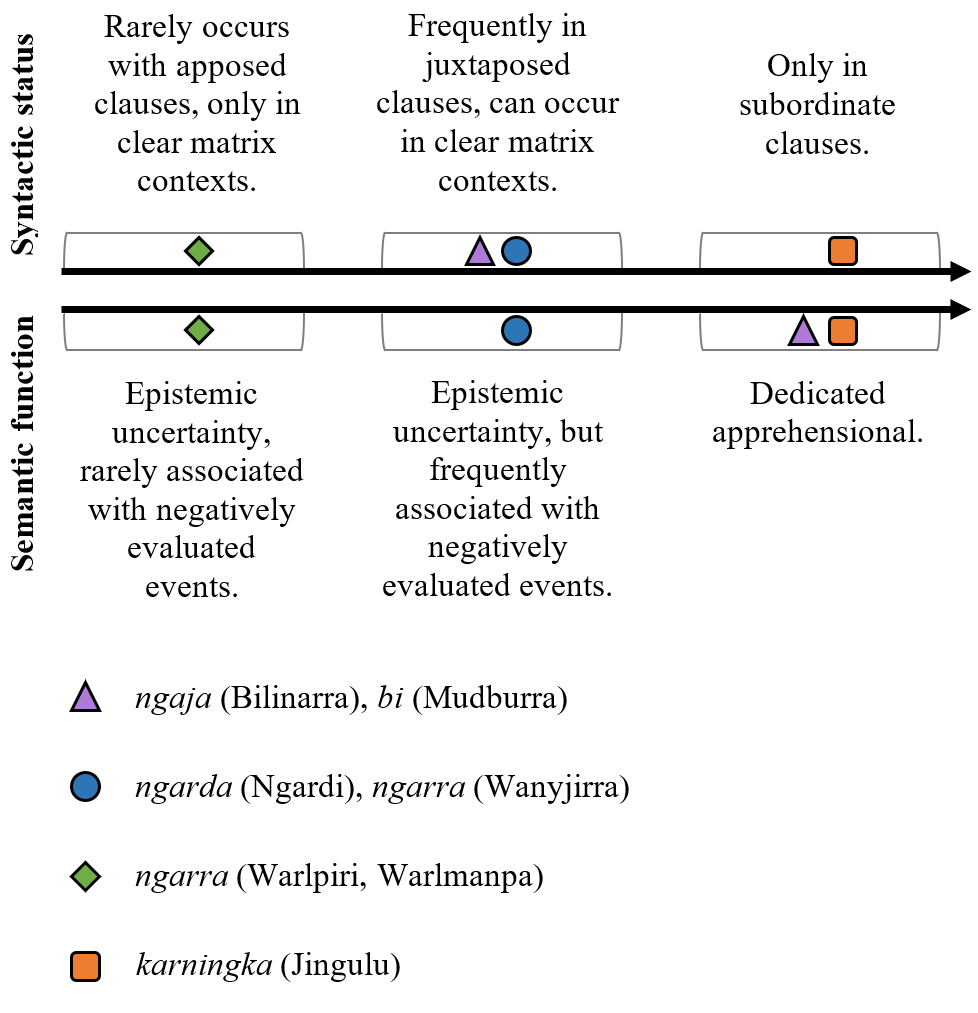
\includegraphics[width=1\textwidth]{figures/figure5browne.png}
    \label{fig5}
\end{figure}

\largerpage
Finally, there are some cases where both a dedicated case morpheme and a non-dedicated auxiliary construction can co-occur as in (\ref{ex:bro71}). In these cases, it seems the apprehensive clause expands upon the negative event associated with the referent -- here the addressees are being taken away for fear of the man, which is a nominal taking the aversive case, followed by a clause which expands upon the negative event associated with the men.


\ea 
\textnormal{\ili{Ngardi} (Western Ngumpin)} \\
\gll Ka-ngku=rna=nyurra \textbf{ngantany-jamarra} \textbf{ngarda}=lu=nganpa luwa-rnngi. \\
carry-\textsc{pot=1sg.s=2pl.ns} \textbf{man-\textsc{ave}} \textsc{\textbf{appr}=3pl.s=1pl.incl.ns} spear-\textsc{irr} \\
\glt `I will take all of you for fear of the men, lest they (the men) spear us.' $[$MRN: LC35b: 322091\_328446$]$
\label{ex:bro71}
\z


\section{Discourse functions}
\label{sec:discourse}

To conclude this paper, we now discuss the discourse functions (speech acts) instantiated by the different apprehensional constructions we have presented. Apprehensional constructions (i.e.\  clauses involving apprehensional morphemes, with or without an overt preemptive clause) in \ili{Ngumpin-Yapa} are frequently associated with two kinds of discourse functions: directives (\sectref{subsec:directives}) and assertives (\sectref{subsec:assertives}). Apprehensional constructions in directive function compel an addressee to some action and entail a negative outcome should the addressee not comply. Apprehensional constructions in assertive function on the other hand are a type of representative speech act that motivates a course of events, again by expression of a less desirable course of events. The primary morphosyntactic correspondences are that apprehensional directives make use of irrealis modalities often with second person subjects (implied or overt), whereas apprehensional assertives make use of realis modalities and describe events which affect participants with any personhood but most frequently first persons -- summarised in \tabref{tab9-bro}.

\begin{table}

\caption{Typical modality and person values for the types of apprehensional constructions in Ngumpin-Yapa languages.}
\label{tab9-bro}
\begin{tabular}{lll}
\lsptoprule
Speech act type & Typical modality & Typical affected participant \\ \midrule
Directive & Irrealis & 2\textsuperscript{nd} (1\textsuperscript{st} person occasionally) \\
Assertives & Realis & Any (1\textsuperscript{st} person most common) \\ 
\lspbottomrule
\end{tabular}
\end{table}


\subsection{Directives}
\label{subsec:directives}

Apprehensional constructions are often associated with directives, either instructing (commands) an addressee to perform some action (or avoid performing some action) in order to avoid an undesirable outcome, or suggesting (entreating) an action to this effect. There are three main morphosyntactic strategies for this. The first two involve either a direct command (imperative clause) or indirect command (potential/irrealis clause) denoting the instructions and an associated apprehensional construction (either a full clause, or a nominal with relational function marked for apprehension). The third is a conditional preemptive clause which signals an event which will lead to an undesired event. These strategies are summarised in \tabref{tab10-bro}, and discussed in more detail below. Interestingly, while the first two types of preemptive clauses can be negated with an associated change of illocutionary meaning (`do/do not do a certain action'), the conditional clause strategy is inherently intended not to be heeded in its positive polarity form (i.e.\  do not perform this action) even without the presence of any clausal negation.

\begin{table}

\caption{Summary of directives involving apprehension.}
\label{tab10-bro}
\begin{tabularx}{\textwidth}{p{19mm}QQ}
\lsptoprule
{Speech act} & {Morphosyntax} & {Expected response} \\
\midrule
Direct \newline command   & Imperative construction and either\newline (i) aversive dependent; or\newline (ii) associated finite apprehensional clause.   & Addressee is expected to\newline perform this action to avoid\newline something undesired.   \\
\tablevspace
Indirect \newline command   & Irrealis verbal inflection and either\newline (i) aversive dependent; or\newline (ii) associated finite apprehensional clause.   & Addressee is encouraged to\newline perform this action to avoid\newline something undesired.   \\
\tablevspace
Conditional \newline warning   & Conditional complementiser \newline with finite matrix \newline apprehensional clause. & Addressee should avoid \newline allowing some action \newline occurring to avoid something \newline undesired.   \\
\lspbottomrule
\end{tabularx}

\end{table}


\subsubsection{Direct command}

An apprehensional construction may involve an overt preemptive clause which serves as a command; its morphosyntactic realisation involves a verb in the imperative inflection. These constructions convey that the addressee is expected (i.e.\  deontic modality) to perform the action denoted by the imperative clause, which will then avoid the undesired entity (for a case marked nominal in an aversive function, as in \REF{ex:bro72}), or avoid an undesired event, as in \REF{ex:bro73}, where the clause containing the predicate is headed by the auxiliary \textit{kala} \textsc{`hab'}.

%\begin{enumerate}
%    \item 
%\newpage
\ea \textnormal{Aversive dependent:} \\
\langinfo{Jaru}{Western Ngumpin}{\citealt[58]{tsunoda_djaru_1981}} \\
\gll Wanyja-rra gardiya-rla! \\
leave-\textsc{imp} white\_man-\textsc{loc} \\
\glt `Leave it for fear of the white man!' 
\label{ex:bro72}
\z
\newpage
%    \item 
\ea \textnormal{Finite apprehensional clause:} \\
\textnormal{\ili{Warlmanpa} (Yapa)} \\
\gll Lamarta-ka jawurra=nya, kala=nga ngapa walikwalik-wa-nmi. \\
hold-\textsc{imp} cup=\textsc{foc} \textsc{appr=pot} water spill-fall-\textsc{fut} \\
\glt `Hold the cup, lest water spill.' $[$wrl-20190205, DK, 34:01$]$
\label{ex:bro73}
\z
%\end{enumerate}

\subsubsection{Indirect command}

Apprehensional constructions may also occur with main clauses that comprise a verb in an irrealis mood and take the form of indirect commands. In these cases, a preemptive clause is realised with irrealis modality (typically through an irrealis inflection, though this is language-dependent), with either an aversive-marked nominal (or non-finite subordinate clause), as in \REF{ex:bro74}, or with a finite clause with an apprehensional auxiliary base, as in \REF{ex:bro75} and \REF{ex:bro76}. Unlike imperatives, the addressee is not deontically \textit{expected} to perform the action referred to by the irrealis clause, but the speaker believes it would be beneficial (typically for the addressee) to do so.


\ea
\langinfo{Walmajarri}{Western Ngumpin} {\citealt{richards_interactive_2012}} \\
\gll Ngajirta nga-n jatpara-karra yan-ta \textbf{purangu-rlamarra}. \\
\textsc{neg} \textsc{mr2-2sg.s} stop-\textsc{mann} go-\textsc{irr} sun-\textsc{ave} \\
\glt `Don't keep stopping, go, for fear of the sun (getting too hot).'
\label{ex:bro74}
\z

\ea 
\textnormal{\ili{Ngardi} (Western Ngumpin)} \\
\gll Wanja-ku=n \textbf{ngarda}=ngkurla wanti-ngi jina-ngka. \\
leave-\textsc{pot=2sg.s} \textsc{\textbf{appr}=2sg.lct} fall-\textsc{irr} foot-\textsc{loc} \\
\glt `You should leave it (the axe) lest it fall on your foot.' [PSM: TEN1-2020\_004-01: 26146\_37777]
\label{ex:bro75}
\z

\ea 
\textnormal{\ili{Ngardi} (Western Ngumpin)} \\
\gll Wakurra=n walya-ngka yirra-ku yawiyi, \textbf{ngarda} wanti-ngi. \\
\textsc{neg=2sg.s} ground-\textsc{loc} place-\textsc{pot} poor\_thing \textbf{\textsc{appr}} fall-\textsc{irr} \\
\glt `You shouldn't put (the kid) down on the ground, he might fall over.' [PSM: TEN1-2020\_006-01: 245249\_252587]
\label{ex:bro76}
\z

 Finally, there are apprehensional constructions where the preemptive clauses are protases of conditionals. In these cases, the matrix clause is marked with the apprehensive auxiliary, and a finite subordinate clause, headed by a conditional, signals an event which will lead to the apprehensive situation eventuating. That is, if the event depicted by the protasis clause becomes true, the undesired event will occur. The inferred directive of these constructions is to \textit{prevent} the event of the conditional clause from unfolding. Unlike the commands detailed above, the conditional warning has a purely inferred directive component. Furthermore, conditional warnings must have a finite apprehensional component (i.e.\  using the apprehensional auxiliary). These can either serve as warnings in specific circumstances, as in \REF{ex:bro77}, or more general warnings about the world, as in \REF{ex:bro78}.

\ea 
\textnormal{\ili{Warlmanpa} (Yapa)} \\
\gll \textbf{Kari}=n kuyu nga-rninjakurla, \textbf{nga}=n=\textbf{nga} murrumurru-ja-ma. \\
\textbf{\textsc{cond}}=\textsc{2sg.s} meat eat-\textsc{cfact} \textbf{\textsc{appr}}=\textsc{2sg.s=\textbf{appr}} sick-\textsc{inch-pot} \\
\glt `If you were to eat this meat, you might become sick.' \\
(Inferred directive: 'Don't eat the meat.') [H\_K01 506A, DG, 04:42]
\label{ex:bro77}
\z

\ea 
\langinfo{Warlpiri}{Yapa}{\citealt[518]{laughren_warlpiri-english_2007}} \\
\gll Nyunypa-ngku ka luwa-rni kiwinyi=ji kuyu nyanungu-ku. Kala \textbf{kaji}=lpa yapa luwa-karla warlura-rlu=ju, ngula=ju \textbf{kalaka} milpa karltara-jarri-mi. \\
saliva-\textsc{erg} \textsc{prs} shoot-\textsc{npst} mosquito=\textsc{top} meat that\_one-\textsc{dat} but \textsc{\textbf{cond}=ipfv} person shoot-\textsc{irr} gecko-\textsc{erg=top} that=\textsc{top} \textsc{\textbf{appr}} eye blind-\textsc{inch-npst} \\
\glt `It spits on mosquitoes which it catches thus to eat. If the gecko hits a person (with its spittle), then the person can go temporarily blind in the eyes.' 
\label{ex:bro78}
\z

 Some Ngumpin languages do not have this conditional apprehensional construction: for example, in \ili{Wanyjirra} and \ili{Ngardi}, for a combination of a conditional subordinate clause with a \textit{ngarda}/\textit{ngarra} marked main clause, the main clause denotes only possibility, and is rarely associated with apprehension, as exemplified in \REF{ex:bro79}--\REF{ex:bro80}.

\ea 
\textnormal{\ili{Ngardi} (Western Ngumpin)} \\
\gll \textbf{Kaji}=rna kuyi ka-ngku-rni kupa-ku \textbf{ngarra}=yi=n. \\
\textsc{\textbf{cond}=1sg.s} meat carry-\textsc{pot-hith} cook-\textsc{pot} \textsc{\textbf{irr}=1sg.ns=2sg.s} \\
\glt `If I bring back this meat, you might cook it for me.' [PSM: TEN1-2020\_006-01: 245249\_252587]
\label{ex:bro79}
\z

\ea 
\langinfo{Wanyjirra}{Western Ngumpin}{\citealt[643]{senge_grammar_2015}} \\
\gll \textbf{Nyanga} maarn yan-gu marri, gangirriny \textbf{ngarra}=ngaliwa garru-wu. \\
\textsc{\textbf{cond}} cloud go-\textsc{fut} off sun \textsc{\textbf{irr}=1aug.inc.ns} stay-\textsc{fut} \\
\glt `When the clouds go away, there will be the sun for us.'
\label{ex:bro80}
\z


 \ili{Mudburra} allows a similar construction, in which the protasis can be apprehensional (marked by the \textit{bi}= auxiliary base). In this case, the condition is something to be avoided, and the main clause signals an action to be undertaken to revert the undesirable event. This is exemplified in \REF{ex:bro81}, where the condition is the addressee forgetting a referent (totemic designs), which is undesired, and the main clause is that the addressee would have to be sure to hold on to the totemic designs. By performing the main clause event under the appropriate conditions (undesired conditions), the addressee reverts to a state where the undesired conditions are no longer met.


\ea 
\langinfo{Mudburra}{Eastern Ngumpin}{\citealt[107]{osgarby_verbal_2018}} \\
\gll $[$Kawarraj \textbf{bi}=n=\textbf{baa} {warnd-arda,$]{_\textnormal{\textsc{condition}}}$ \hspace*{2cm}} $[$nya=n durd ma-rrarnda wumangku=ma.$]{_\textnormal{\textsc{result}}}$ \\
forget \textsc{\textbf{appr}=2sg.s=\textbf{cond}} get-\textsc{sbjv} \textsc{appr=2sg.s} hold do-\textsc{sbjv} dreaming=\textsc{top} \\
\glt `If you were in danger of forgetting them, you would have to hold on to your totemic designs.'
\label{ex:bro81}
\z

\subsection{Assertives}
\label{subsec:assertives}
\largerpage

Apprehensional constructions in \ili{Ngumpin-Yapa} languages are also used as assertives, in particular providing the reasoning behind a speaker’s actions. Examples are given in \REF{ex:bro82}--\REF{ex:bro85} which demonstrate the wide range of temporal references permitted in the preemptive clause: the example in \REF{ex:bro82} has present reference; \REF{ex:bro83} has past reference; and finally \REF{ex:bro84}--\REF{ex:bro86} have future reference. The apprehensional component, either a finite clause with an apprehensive auxiliary and irrealis modality, or a nominal with aversive case marking (or a non-finite subordinate clause with aversive case marking), obtains its temporal reference from the preemptive clause.

\ea
\textnormal{\ili{Ngardi} (Western Ngumpin)} \\
\gll Ngu=rna jaku=ya-nanta, \textbf{ngarda}=yi=lu paja-rnngi kunyarr-u. \\
\textsc{seq=1sg.s} depart=go\textsc{-prs} \textsc{\textbf{appr}=1sg.ns=3pl.s} bite-\textsc{irr} dog-\textsc{erg} \\
\glt `I'm getting out of here, \textbf{lest} those dogs bite me!' [PSM: TEN1-2017\_010-01: 954694\_959466]
\label{ex:bro82}
\z

\ea 
\textnormal{\ili{Ngardi} (Western Ngumpin)} \\
\gll Ngu=lu=yanu wiriny=ma-ni yard-ta=wali ngantany jayin-kurlu jina \textbf{ngarda}=lu yaparti-ngi. \\
\textsc{seq=3pl.s=3pl.ns} bind=get-\textsc{pst} yard-\textsc{loc}=then man chains-\textsc{prop} foot \textsc{\textbf{appr}=3pl.s} run-\textsc{irr} \\
\glt `They tied the aboriginal men up in the yard (by their) feet with chains, lest they flee.' [PSM: TEN1-2017\_007-02: 72766\_82623]
\label{ex:bro83}
\z

\ea 
\textnormal{\ili{Ngardi} (Western Ngumpin)} \\
\gll Ya-nku=rna yalu-rlamarra, \textbf{ngarda}=yirla wangka-nyanku. \\
go-\textsc{pot=1sg.s} that-\textsc{ave} \textsc{\textbf{appr}=1sg.lct} speak-\textsc{ipfv.pot} \\
\glt `I will go on account of that one, lest she speak with me.' [MMN: TEN1-2017\_026-01: 1168486 \_1207635]
\label{ex:bro84}
\z

\ea 
\textnormal{\ili{Warlmanpa} (Yapa)} \\
\gll \textbf{Ngapa}-\textbf{kuma}=rna mulpu-nga purluny-ya-n. \\
\textbf{water-\textsc{ave}}=\textsc{1sg.s} shelter-\textsc{loc} enter-go-\textsc{fut}  \\
\glt `I will enter shelter for fear of the rain.' [H\_K01 506A, DG, 39:05]
\label{ex:bro85}
\z

\largerpage
 Apprehensional constructions can be used not in reference to a specific event but rather to justify claims about generally observed behaviours or phenomena. In \REF{ex:bro86}, a speaker claims that cars cannot go over sandhills, the justification being that the car will get bogged, which is marked with apprehensional morphology.

\ea
\langinfo{Warlpiri}{Yapa}{\citealt[116]{laughren_warlpiri-english_2007}} \\
\gll Jilja ka pirli=piya parntarri-nja-ya-ni kula=lpa  murduka=yi jilja-ngka ya-ntarla, lawa --- \textbf{kalaka} yuka-mi. \\
sandhill \textsc{prs} rock=\textsc{sembl} crouch-\textsc{inf}-go-\textsc{npst} \textsc{neg=ipfv} car=\textsc{cont} sandhill-\textsc{loc} go-\textsc{irr} \textsc{neg} \phantom{---} \textsc{\textbf{appr}} sink-\textsc{npst} \\
\glt `A sandhill stretches out like a rocky mesa---a car can't go over a sandhill, as it's likely to get bogged.'
\label{ex:bro86}
\z

\section{Conclusion}

This chapter has provided the first in-depth analysis of apprehensional constructions of \ili{Ngumpin-Yapa} languages. These languages exhibit a case suffix which can mark a nominal denoting a feared referent (or a feared event metonymically associated with a referent), or it can mark a non-finite subordinate clause denoting a feared event. In some cases it is difficult to distinguish which particular function is instantiated in a given utterance, which is a common analytical problem in Australian languages \citep{hale_essential_1982}. While most \ili{Ngumpin-Yapa} languages have this construction available, few use the aversive case suffix to mark the complement of a `fear' predicate, and it is more common to mark these complements using dative or locative suffixes which still trigger verbal indexation (thus distinct from adjunct uses of the dative and locative cases). In most \ili{Ngumpin-Yapa} languages, the form of the aversive suffix is an increment to another case (particularly dative, as in \ili{Warlmanpa}, or locative, as in \ili{Ngardi}), which can be seen in other Australian languages as well (e.g.\  \ili{Pintupi}).

Most \ili{Ngumpin-Yapa} languages also have an auxiliary which marks finite clauses as denoting undesired eventualities -- while this has been found in non-Pama-Nyungan languages, this is rare for \ili{Pama-Nyungan} languages. There is great interlanguage variation as to whether these auxiliaries are more like complementisers (i.e.\  in these languages, these constructions rely on a matrix preemptive clause), and to the extent to which these auxiliaries exclusively encode apprehension or whether other interpretations are available. Generally, these other interpretations are general irrealis meanings, which leaves available an apprehensive interpretation. This variation indicates that within these languages, apprehension is not a diachronically stable phenomenon, particularly striking in one form which appears to be a shared inherited form \textit{ngaCa} which is dedicated to apprehensional meanings in some languages but has a more general irrealis function in others, as well as exhibiting variance regarding its syntactic status. Furthermore, the interpretation of apprehension is tied to the verb inflection, as well as the auxiliary. Finally, the chapter discussed the most common usage of apprehensional constructions: directives of varying strength, and assertives, which primarily provide the reasoning for a speaker's actions. 


\section*{Abbreviations}
\begin{tabularx}{.5\textwidth}{@{}lQ@{}}
\textsc{1/2/3} & 1st/2nd/3rd person \\
\textsc{A} & Agent\\
\textsc{abl} & ablative \\
\textsc{abs} & absolutive \\
\textsc{acc} & accusative \\
\textsc{acs} & accessory \\
\textsc{adm} & admonitive\\
\textsc{all} & allative\\
\textsc{anaph.prop} & anaphoric/reflexive pronoun \end{tabularx}
\begin{tabularx}{.5\textwidth}{@{}lQ@{}}
\textsc{antic} & anticipatory \\
\textsc{appr} & apprehensive \\
\textsc{aug} & augmented \\
\textsc{aux} & auxiliary\\
\textsc{ave} & aversive \\
\textsc{cat} & catalyst \\
\textsc{caus} & causative \\
\textsc{cfact} & counterfactual \\
\textsc{com} & comitative\\
\textsc{cond} & conditional \end{tabularx}
\begin{tabularx}{.5\textwidth}{@{}lQ@{}}
\textsc{cont} & continuous \\
\textsc{cust} & customary aspect \\
DD & daughter's daughter\\
\textsc{dat} & dative\\
\textsc{dist} & distal demonstrative\\
\textsc{d.loc} & derivational locative \\\
\textsc{du} & dual\\
\textsc{dub} & dubitative \\
\textsc{eff} & effector \\
\textsc{erg} & ergative \\
\textsc{excl} & exclusive \\
\textsc{foc} & focus \\
\textsc{fut} & future \\
\textsc{hab} & habitual\\
\textsc{hith} & hither \\
\textsc{hyp} & hypothetical\\
\textsc{imp} & imperative \\
\textsc{incl} & inclusive\\
\textsc{inch} & inchoative \\
\textsc{inf} & infinitive \\
\textsc{inst} & instrumental \\
\textsc{ipfv} & imperfective \\
\textsc{lest} & `lest'; apprehensional marker \\
\textsc{irr} & irrealis \\
\textsc{lct} & locational \\
\textsc{link} &  linker\\
\textsc{loc} & locative \\
\textsc{mann} & manner \\
\textsc{min} & minimal \\
MM & mother's mother\\
\textsc{mot} & associated motion \end{tabularx}
\begin{tabularx}{.5\textwidth}{@{}lQ@{}}
\textsc{mr1/2/3} & modal root 1/2/3 \\
\textsc{narr} & narrative\\
\textsc{neg} & negative \\
\textsc{nmlz} & nominalizer \\
\textsc{npst} & non-past \\
\textsc{nom} & nominative \\
\textsc{ns} & non-subject \\
\textsc{o} & object \\
\textsc{obl} & oblique \\
\textsc{obsc} & obscured \\
\textsc{passp} & passive perfective \\
\textsc{perf} & perfect \\
\textsc{pl} & plural\\
\textsc{pot} & potential\\
\textsc{prep} & preparative \\
\textsc{prop} & proprietive (`having') \\
\textsc{prs} & present \\
\textsc{pst} & past \\
\textsc{rdp} & reduplication \\
\textsc{purp} & purposive \\
\textsc{real} & realis \\
\textsc{refl} & reflexive\\
\textsc{rstr} & restrictive \\ 
\textsc{s} & subject\\
\textsc{sbjv} & subjunctive \\
\textsc{sembl} & semblative \\
\textsc{sg} & singular \\
\textsc{spec} & speculative \\
TAM & tense, aspect, mood\\
\textsc{top} & topic \\
\textsc{vblsr} & verbaliser
\end{tabularx}


\printbibliography[heading=subbibliography,notkeyword=this]
\end{document}
